\thispagestyle{thachthuctoanhocnone}
\pagestyle{thachthuctoanhoc}
\everymath{\color{thachthuctoanhoc}}
\graphicspath{{../thachthuctoanhoc/pic/}}
\begingroup
\AddToShipoutPicture*{\put(0,616){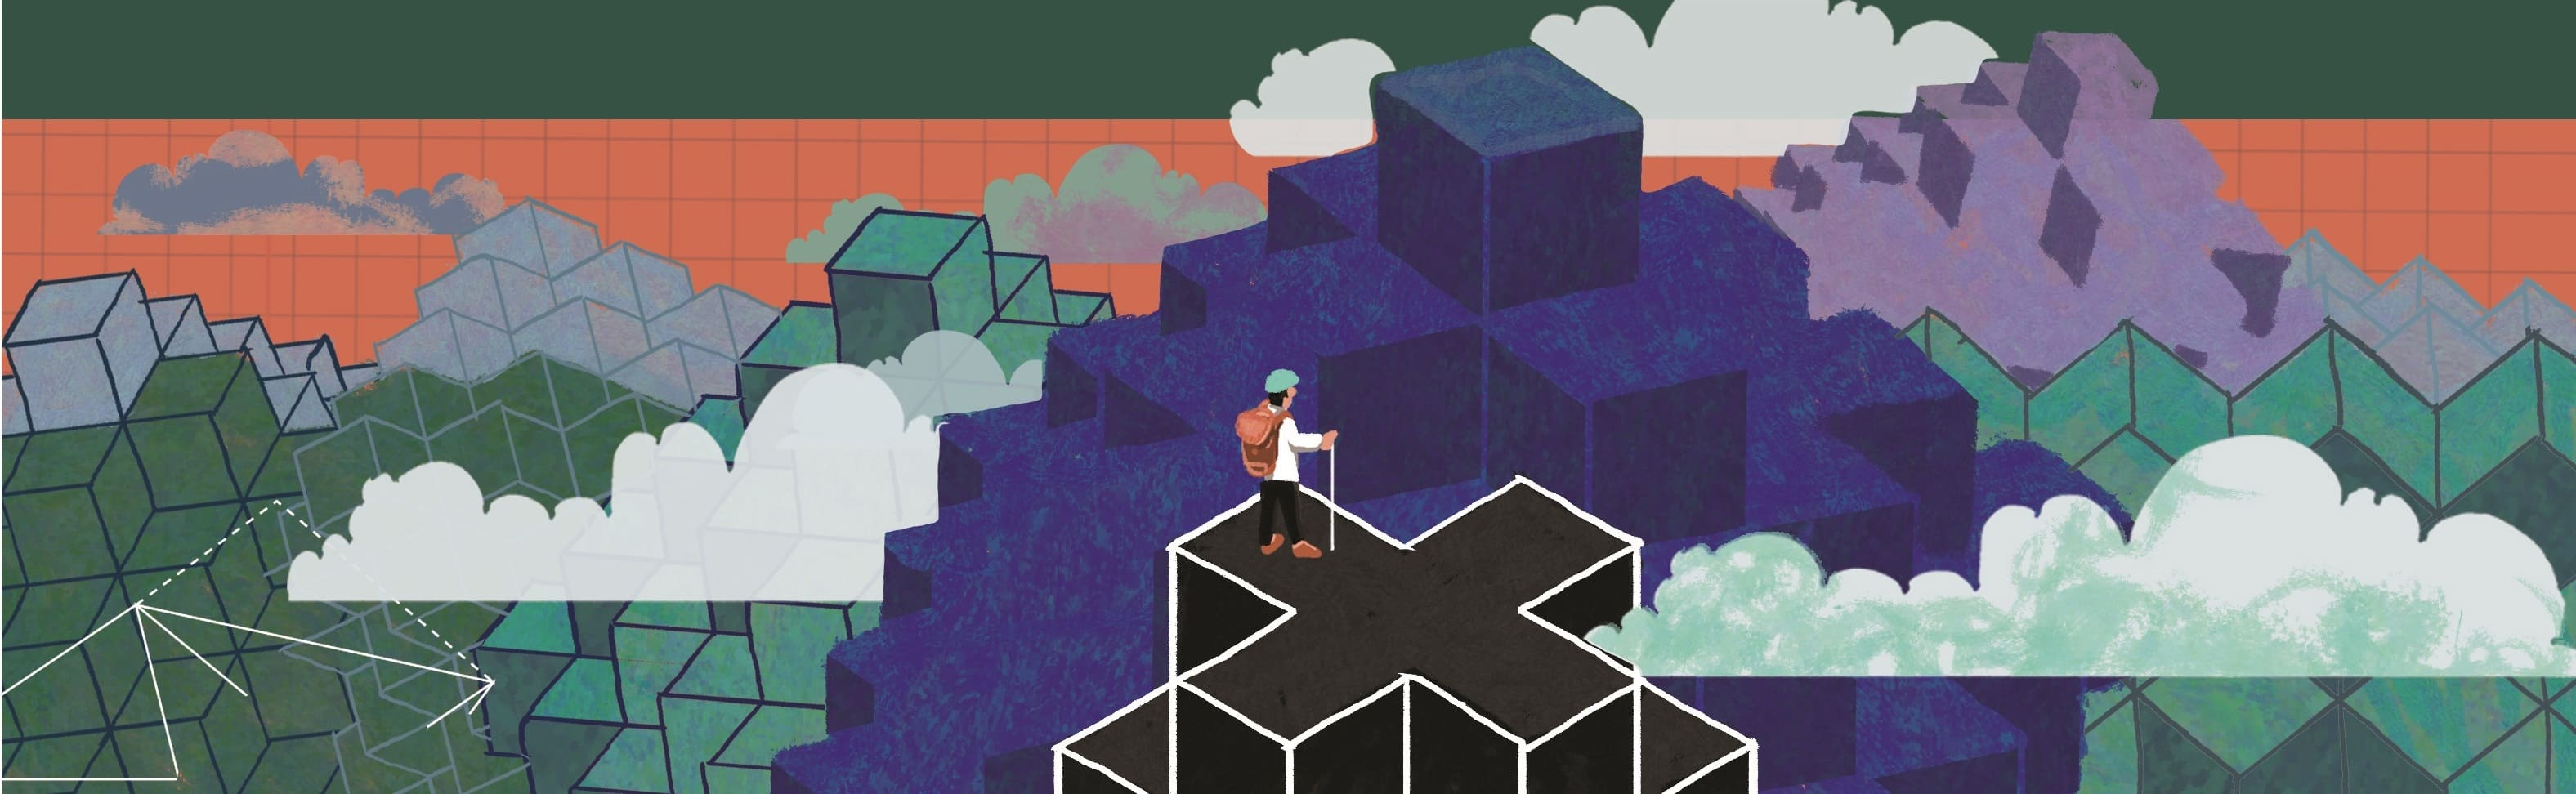
\includegraphics[width=19.3cm]{../thachthuctoanhoc/bannerthachthuc}}}
\centering
\vspace*{4cm}
\endgroup
\vspace*{-8pt}
\begin{tBox}
	\begin{itemize}[leftmargin = 13pt, itemsep = 1.0pt] 
		\item Mỗi bài toán đề xuất (kèm theo lời giải) cần được nêu rõ là bài sáng tác hay bài sưu tầm.
%				\item Mỗi bài toán đề xuất (kèm theo lời giải) cần được nêu rõ là bài sáng tác hay bài sưu tầm (nếu là bài sưu tầm, cần ghi rõ nguồn).
		\item Bài giải cho mỗi bài toán cần được trình bày trong một file riêng hoặc
		một tờ giấy riêng.
		\item  Người đề xuất bài toán hoặc gửi bài giải cho các bài toán trong mục ``Thách thức kỳ này" cần ghi rõ họ, đệm, tên và nơi làm việc/học tập, số điện thoại liên hệ. Nếu là học sinh (hoặc sinh viên) cần ghi rõ là học sinh lớp mấy (hoặc sinh viên năm thứ mấy).
		\item Các bài toán trong mục Thách thức kỳ này hướng tới các độc giả là học sinh phổ thông; được phân chia thành các mức độ $B$, $A$, và được sắp xếp theo độ khó tăng dần, theo đánh giá chủ quan của Ban biên tập. Các bài toán mức độ $B$ không đòi hỏi các kiến thức vượt quá chương trình môn Toán cấp THCS; các bài toán mức độ $A$ không đòi hỏi các kiến thức vượt quá chương trình môn Toán cấp THPT.
		\item Cách thức gửi bài toán đề xuất hoặc lời giải: gửi file thu được bằng cách scan, ảnh chụp (rõ nét) của bản viết tay, hoặc được soạn thảo bằng các phần mềm Latex, Word tới \url{bbt@pi.edu.vn} hoặc gửi qua đường bưu điện tới Tòa soạn (xem địa chỉ tại bìa $2$).
		\item Hạn gửi lời giải cho các bài toán P$691$--P$700$: trước ngày $15/5/2023$.
	\end{itemize}
\end{tBox}
\begin{center}
	\vspace*{-5pt}
	\textbf{\color{thachthuctoanhoc}\color{thachthuctoanhoc}\color{thachthuctoanhoc}THÁCH THỨC KỲ NÀY}
	\vspace*{-5pt}
\end{center}
\begin{multicols}{2}
	\setlength{\abovedisplayskip}{4pt}
	\setlength{\belowdisplayskip}{4pt}
	{\color{thachthuctoanhoc}{\usefont{T5}{qag}{b}{n} P691.}}
	(Mức $B$) Tìm tất cả các số có sáu chữ số, trong đó chữ số hàng trăm nghìn bằng $\dfrac16$ tổng năm chữ số còn lại; chữ số hàng chục nghìn bằng $\dfrac16$  tổng bốn chữ số nằm bên phải nó.
	\vskip 0.05cm
	\hfill	\textit{\small Duy Minh, Hà Nội (st)}
	\vskip 0.05cm
	{\color{thachthuctoanhoc}{\usefont{T5}{qag}{b}{n} P692.}}
	(Mức $B$)  Ở mỗi ô vuông con của bảng ô vuông kích thước $3\times3$, có $4$ viên bi. Bạn Hà lấy bi ra khỏi bảng, theo quy tắc: Mỗi lần, lấy hai viên bi nằm ở hai ô vuông con kề nhau, ở mỗi ô lấy một viên. Hỏi, bạn Hà có thể lấy ra khỏi bảng tối đa bao nhiêu viên bi?
	\vskip 0.05cm
	({\it Hai ô vuông được gọi là kề nhau, nếu chúng có cạnh chung}.)
	\begin{flushright}
		\textit{\small Trích Đề thi VMTC $2022$--Vòng $2$--Khối lớp $8$}
	\end{flushright}
	{\color{thachthuctoanhoc}{\usefont{T5}{qag}{b}{n} P693.}}
	(Mức $B$) Cho các số thực phân biệt $a,b,c$  thoả mãn
	\begin{align*}
		\dfrac{(a+b)(b+c)(c+a)}{(a-b)(b-c)(c-a)}=\dfrac{23}{20}.
	\end{align*}
	Tính
	\begin{align*}
		S=\dfrac{a}{a+b}+\dfrac{b}{b+c}+\dfrac{c}{c+a}.
	\end{align*}
	\begin{flushright}
		\textit{\small Trích Đề thi VMTC $2022$--Vòng $2$--Khối lớp $8$}
	\end{flushright}
	{\color{thachthuctoanhoc}{\usefont{T5}{qag}{b}{n} P694.}}
	(Mức $B$) Cho tập hợp $S$ gồm tất cả các số tự nhiên có ba chữ số. Chứng minh rằng, trong $106$ số đôi một khác nhau tùy ý thuộc $S$, luôn tồn tại $8$ số, sao cho có thể phân chia $8$ số này thành $4$ nhóm, mỗi nhóm có hai số, và các tổng hai số cùng nhóm bằng nhau.
	\begin{flushright}
		\textit{\small Trích Đề thi VMTC $2022$--Vòng $2$--Khối lớp $8$}
	\end{flushright}
	{\color{thachthuctoanhoc}{\usefont{T5}{qag}{b}{n} P695.}}
	(Mức $B$) Tìm tất cả các cặp số tự nhiên $(x;y)$ thoả mãn $x^2+16=5^y$. 
	\vskip 0.05cm
	\hfill\textit{\small Trích Đề thi VMTC $2022$--Vòng $2$--Khối lớp $9$}
	\vskip 0.05cm
	{\color{thachthuctoanhoc}{\usefont{T5}{qag}{b}{n} P696.}}
	(Mức $B$) Cho lục giác đều $ABCDEF$ có cạnh bằng $1$ và $M$ là một điểm tuỳ ý nằm trong lục giác đó. Chứng minh rằng, trong $6$ tam giác $MAB$, $MBC$, $MCD$, $MDE$, $MEF$ và $MFA$ có ít nhất $3$ tam giác có chu vi không nhỏ hơn $3$. 
	\begin{figure}[H]
		\vspace*{-15pt}
		\centering
		\captionsetup{labelformat= empty, justification=centering}
		\definecolor{qqzzff}{rgb}{0,0.6,1}
		\definecolor{zzttqq}{rgb}{0.6,0.2,0}
		\definecolor{qqqqff}{rgb}{0,0,1}
		\definecolor{qqqqffa}{rgb}{1,1,1}
		\begin{tikzpicture}[thachthuctoanhoc,scale=0.55]
			\draw [color=qqzzff] (-1.092089618842777,3.780911308935779)-- (2.5235020561954022,3.780911308935779);
			\draw [color=qqzzff] (2.5235020561954022,3.780911308935779)-- (4.331297893714492,6.912105549230374);
			\draw [color=qqzzff] (4.331297893714492,6.912105549230374)-- (2.5235020561954027,10.04329978952497);
			\draw [color=qqzzff] (2.5235020561954027,10.04329978952497)-- (-1.0920896188427762,10.04329978952497);
			\draw [color=qqzzff] (-1.0920896188427762,10.04329978952497)-- (-2.8998854563618672,6.912105549230376);
			\draw [color=qqzzff] (-2.8998854563618672,6.912105549230376)-- (-1.092089618842777,3.780911308935779);
			\draw  (-1.092089618842777,3.780911308935779)-- (0.9849524072429845,5.223301604828669);
			\draw  (0.9849524072429845,5.223301604828669)-- (2.5235020561954022,3.780911308935779);
			\draw  (0.9849524072429845,5.223301604828669)-- (4.331297893714492,6.912105549230374);
			\draw  (0.9849524072429845,5.223301604828669)-- (-2.8998854563618672,6.912105549230376);
			\draw  (0.9849524072429845,5.223301604828669)-- (-1.0920896188427762,10.04329978952497);
			\draw  (0.9849524072429845,5.223301604828669)-- (2.5235020561954027,10.04329978952497);
			\draw [fill=white] (-1.092089618842777,3.780911308935779) circle (1.5pt);
			\draw[color=qqqqff] (-1.284408324961828,3.1597447968988694) node {$A$};
			\draw [fill=white] (2.5235020561954022,3.780911308935779) circle (1.5pt);
			\draw[color=qqqqff] (2.523502056195404,3.15597447968988694) node {$B$};
			\draw [fill=white] (4.331297893714492,6.912105549230374) circle (1.5pt);
			\draw[color=qqqqff] (4.7500544082281167,7.079177118877521) node {$C$};
			\draw [fill=white] (2.5235020561954027,10.04329978952497) circle (1.5pt);
			\draw[color=qqqqff] (2.65812515047874,10.425522605349025) node {$D$};
			\draw [fill=white] (-1.0920896188427762,10.04329978952497) circle (1.5pt);
			\draw[color=qqqqff] (-1.284408324961828,10.425522605349025) node {$E$};
			\draw [fill=white] (-2.8998854563618672,6.912105549230376) circle (1.5pt);
			\draw[color=qqqqff] (-3.3037547392118753,7.002249636429901) node {$F$};
			\draw [fill=white] (0.9849524072429845,5.223301604828669) circle (1.5pt);
			\draw[color=qqqqff] (0.8887930541834608,4.681202135092791759) node {$M$};
		\end{tikzpicture}
		\vspace*{-15pt}
	\end{figure}
	\hfill	\textit{\small Nguyễn Văn Bản, Điện Biên}
	\vskip 0.05cm
	{\color{thachthuctoanhoc}{\usefont{T5}{qag}{b}{n} P697.}}
	(Mức $A$) Cho các số dương $x,y,z$ thoả mãn $x^2+y^2+z^2=3$. Chứng minh rằng
	\begin{align*}
		\sqrt[3]{\dfrac{y z}{x^5\!-\!x\!+\!8}}\!+\!\sqrt[3]{\dfrac{z x}{y^5\!-\!y\!+\!8}}\!+\!\sqrt[3]{\dfrac{x y}{z^5\!-\!z\!+\!8}} \!\le\! \dfrac{3}{2}.
	\end{align*}
	\hfill \textit{Hoàng Lê Nhật Tùng, Hà Nội}
	\vskip 0.05cm
	{\color{thachthuctoanhoc}{\usefont{T5}{qag}{b}{n} P698.}}
	(Mức $A$) Cho số nguyên $m>1$. Chứng minh rằng
	\vskip 0.05cm
	$a)$ Tồn tại $m$ số thực dương $x_1,\ldots,x_m$, không đồng thời bằng $1$, sao cho
	\begin{align*}
		\sqrt[n]{x_1}+\cdots+\sqrt[n]{x_m}
	\end{align*}
	là số nguyên, với mọi $n=1,2,\ldots,100$.
	\vskip 0.05cm
	$b)$ Không tồn  tại $m$ số thực dương $x_1,\ldots,x_m$, không đồng thời bằng $1$, sao cho
	\begin{align*}
		\sqrt[n]{x_1}+\cdots+\sqrt[n]{x_m}
	\end{align*}
	là số nguyên, với mọi số nguyên dương $n$.
	\vskip 0.05cm
	\hfill	\textit{\small Nguyễn Huy Hoàng, Bình Định}
	\vskip 0.05cm
	\columnbreak
	{\color{thachthuctoanhoc}{\usefont{T5}{qag}{b}{n} P699.}}
	(Mức $A$) Cho tam giác không cân $ABC$ nội tiếp đường tròn $(O)$ và có hai đường cao $BE,CF$ cắt nhau tại $H$. Giả sử   $\angle BAC$ khác $60^\circ,90^\circ$ và $120^\circ$.  Gọi $P, Q$ là các điểm, tương ứng, đối xứng với $B,C $ qua $F, E$. Các đường thẳng $HP, HQ$, tương ứng, cắt $AC, AB$ tại $M, N$.  Gọi $K$ là trung điểm của $BC$. Chứng minh rằng, các điểm $M, N, P, Q$ cùng thuộc một đường tròn có tâm nằm trên đường thẳng $HK$.
	\begin{figure}[H]
		\vspace*{-15pt}
		\centering
		\captionsetup{labelformat= empty, justification=centering}
		\definecolor{qqqqff}{rgb}{0,0,1}
		\definecolor{qqqqffa}{rgb}{1,1,1}
		\begin{tikzpicture}[thachthuctoanhoc,scale=0.65]
			\draw  (-0.27473499999999995,6.521887994397557) circle (3.8233413036603774cm);
			\draw  (-1.9190600551547001,9.973573645969253)-- (-3.68839,4.8);
			\draw  (-3.68839,4.8)-- (3.13892,4.8);
			\draw  (3.13892,4.8)-- (-1.9190600551547001,9.973573645969253);
			\draw  (-3.68839,4.8)-- (-0.19761156573467797,8.212783678306042);
			\draw  (-2.973484746555942,6.8904043303842535)-- (3.13892,4.8);
			\draw  (-3.534143131469356,11.625567356612084)-- (-1.9190600551547001,9.973573645969253);
			\draw  (-2.474847925491419,10.542063329077637)-- (-1.919060055154701,6.529797657174141);
			\draw  (-3.534143131469356,11.625567356612084)-- (-1.919060055154701,6.529797657174141);
			\draw [dashed] (-4.685663359168936,9.440209986300777) circle (2.47017927907576cm);
			\draw [dashed] (-4.685663359168939,9.44020998630077)-- (-0.27473499999999995,4.8);
			\draw [fill=white] (-1.9190600551547001,9.973573645969253) circle (1.5pt);
			\draw[color=qqqqff] (-1.72146890661847,10.48321821718474) node {$A$};
			\draw [fill=white] (-3.68839,4.8) circle (1.5pt);
			\draw[color=qqqqff] (-4.0153339518523685,4.579033939329845) node {$B$};
			\draw [fill=white] (3.13892,4.8) circle (1.5pt);
			\draw[color=qqqqff] (3.3889362337311386,4.579033939329845) node {$C$};
			\draw [fill=white] (-0.19761156573467797,8.212783678306042) circle (1.5pt);
			\draw[color=qqqqff] (0.13433673518798938,8.502335544158505) node {$E$};
			\draw [fill=white] (-2.973484746555942,6.8904043303842535) circle (1.5pt);
			\draw[color=qqqqff] (-3.3037547392118753,7.04071337765371) node {$F$};
			\draw [fill=white] (-1.919060055154701,6.529797657174141) circle (1.5pt);
			\draw[color=qqqqff] (-2.1113787612737522,5.8974811953692) node {$H$};
			\draw [fill=white] (-2.258579493111884,8.980808660768506) circle (1.5pt);
			\draw[color=qqqqff] (-1.9575237963785104,8.944668568232325) node {$P$};
			\draw [fill=white] (-3.534143131469356,11.625567356612084) circle (1.5pt);
			\draw[color=qqqqff] (-3.2691602808380743,12.098695348584778) node {$Q$};
			\draw [fill=white] (-2.474847925491419,10.542063329077637) circle (1.5pt);
			\draw[color=qqqqff] (-2.1229293380047094,10.84862375881094) node {$M$};
			\draw [fill=white] (-2.48555043367752,8.31713884614052) circle (1.5pt);
			\draw[color=qqqqff] (-2.8806535857499607,8.4831036735466) node {$N$};
			\draw [fill=white] (-0.27473499999999995,6.521887994397557) circle (1.5pt);
			\draw[color=qqqqff] (-0.11126421763561023,6.829162800922753) node {$O$};
			\draw [fill=white] (-0.27473499999999995,4.8) circle (1.5pt);
			\draw[color=qqqqff] (-0.3420466649784728,4.252133832749413) node {$K$};
			\draw [fill=white] (-4.685663359168939,9.44020998630077) circle (1.5pt);
		\end{tikzpicture}
		\vspace*{-20pt}
	\end{figure}
	\hfill	\textit{\small Lưu Công Đông, Hà Nội}
	\vskip 0.05cm
	{\color{thachthuctoanhoc}{\usefont{T5}{qag}{b}{n} P700.}}
	(Mức $A$) Cho số nguyên dương $n$. Lần lượt ghi các số $n^3,$ $n^3+1,\ldots,$ $n^3+n$ lên $n+1$ tấm thẻ trắng, trên mỗi thẻ ghi đúng một số. Người ta xếp tất cả $n+1$ tấm thẻ đó vào hai chiếc hộp xanh và đỏ, sao cho mỗi hộp có ít nhất một thẻ và  tổng các số được ghi ở các thẻ trong hộp xanh chia hết cho tổng các số được ghi ở các thẻ trong hộp đỏ. Chứng minh rằng, số các tấm thẻ trong hộp xanh chia hết cho số các tấm thẻ trong hộp đỏ.
	\vskip 0.05cm
	\hfill	\textit{\small Tô Trung Hiếu, Nghệ An (st)}
\end{multicols}
\centerline{{\large{\textbf{\color{thachthuctoanhoc}GIẢI BÀI KỲ TRƯỚC}}}}
\vspace*{-5pt}
\begin{multicols}{2}
	\setlength{\abovedisplayskip}{4pt}
	\setlength{\belowdisplayskip}{4pt}
	{\color{thachthuctoanhoc}{\usefont{T5}{qag}{b}{n} P671.}}
	(Mức $B$) Một hình chữ nhật được chia thành $9$ hình chữ nhật con như hình vẽ. Số ghi ở giữa mỗi hình chữ nhật con bằng chu vi của hình chữ nhật ấy. Biết rằng $c$ là một số nguyên khác $2,3,4,5$; hãy tìm $a,b,c,d,e$.
	\begin{center} 
		\definecolor{cqcqcq}{rgb}{0.7529411764705882,0.7529411764705882,0.7529411764705882}
		\begin{tikzpicture}[scale=0.7,thachthuctoanhoc]
			\draw (0,0) rectangle (9,3); 
			\draw (2,0) -- (2, 3) (6, 0) -- (6, 3);
			\draw (0,1.2) -- (9, 1.2) (0, 2.1) -- (9, 2.1);
			\draw (1,2.5) node{$a$};
			\draw (1,1.5) node{$2$};
			\draw (1,0.5) node{$d$};
			\draw (4,2.5) node{$4$};
			\draw (4,1.5) node{$c$};
			\draw (4,0.5) node{$5$};
			\draw (7.5,2.5) node{$b$};
			\draw (7.5,1.5) node{$3$};
			\draw (7.5,0.5) node{$e$};
		\end{tikzpicture}
	\end{center}
	\textbf{\color{thachthuctoanhoc}Lời giải} (\textit{dựa theo lời giải của bạn Hà Mạnh Hùng, lớp $8$A, trường THPT chuyên Hà Nội -- Amsterdam, Tp. Hà Nội})\textbf{\color{thachthuctoanhoc}.}
	\vskip 0.05cm
	Trước hết, ta có Nhận xét đơn giản sau:
	\vskip 0.05cm
	\textbf{\color{thachthuctoanhoc}\textit{Nhận xét.}} Nếu một hình chữ nhật được phân chia thành bốn hình chữ nhật I, II, III, IV như ở hình dưới đây, thì tổng chu vi của hai hình chữ nhật I và IV bằng tổng chu vi của hai hình chữ nhật II và III.
	\begin{figure}[H]
		\vspace*{-5pt}
		\centering
		\captionsetup{labelformat= empty, justification=centering}
		\begin{tikzpicture}[thachthuctoanhoc]
			\draw (0,0) rectangle (5,2.5);
			\draw (0,1.5) -- (5,1.5) (2,0) -- (2,2.5);
			\draw (1,0.75) node{III};	
			\draw (1,2) node{I};
			\draw (3.5,0.75) node{IV};
			\draw (3.5,2) node{III};	
		\end{tikzpicture}
		\vspace*{-10pt}
	\end{figure}
	Theo Nhận xét trên, từ các giả thiết của bài ra về chu vi của $9$ hình chữ nhật con, ta có:
	\begin{align*}
		\quad\quad\begin{cases}
			a + c = 4 + 2 = 6 \hspace*{67pt} (1)\\
			b + c = 4 + 3 = 7 \hfill (2)\\
			c + e = 3 + 5 = 8 \hfill (3)\\
			c + d = 2 + 5 = 7. \hfill (4)
		\end{cases}
	\end{align*}
	Từ ($1$), do $a > 0$, suy ra $0 < c < 6$. Mà $c$ là một số nguyên, khác $2$, $3$, $4$, $5$ (giả thiết), nên $c = 1$. Từ đây và ($1$), ($2$), ($3$), ($4$), lần lượt suy ra, $a = 6 – 1 = 5$, $b = 7 – 1 = 6$, $e = 8 – 1 = 7$, $d = 7 – 1 = 6$.
	\vskip 0.05cm
	Vậy, $a = 5$, $b = 6$, $c = 1$, $d = 6$, $e = 7$.
	\vskip 0.05cm
	\textbf{\color{thachthuctoanhoc}Bình luận và Nhận xét}
	\vskip 0.05cm
	Trong số các lời giải Tạp chí đã nhận được, rất tiếc, có một lời giải không được coi là lời giải hoàn chỉnh, do người giải bài vẫn đang dang dở trong các lập luận lý giải cho kết quả tìm được.
	\begin{flushright}
		\textbf{\color{thachthuctoanhoc}Lê Huy}
	\end{flushright}
	{\color{thachthuctoanhoc}{\usefont{T5}{qag}{b}{n} P672.}}
	(Mức $B$) Cho $x$ và $y$ là các số nguyên dương phân biệt thoả mãn
	\begin{align*}
		2023x^{2023}+999 y^{2023}
	\end{align*}
	chia hết cho $x+y$. Chứng minh rằng $x+y$ là hợp số. 
	\vskip 0.05cm
	\textbf{\color{thachthuctoanhoc}Lời giải} (\textit{phỏng theo Đáp án của bài toán})\textbf{\color{thachthuctoanhoc}.}
	\vskip 0.05cm
	Ta có:
	\begin{align*}
		&2023{x^{2023}} + 999{y^{2023}} \\
		= \,\,&999\left( {{x^{2023}} + {y^{2023}}} \right) + {2^{10}} \cdot {x^{2023}}.
	\end{align*}
	Do $2023$ là số lẻ, nên $\left( {{x^{2023}} + {y^{2023}}} \right) \vdots \left( {x + y} \right)$. Vì thế, từ giả thiết của bài toán và ($1$), suy ra
	\begin{align*}
		{2^{10}} \cdot {x^{2023}} \,\vdots \left( {x + y} \right).
	\end{align*}
	Vì $x, y$ là hai số nguyên dương phân biệt, nên $x + y \ge  3 > 1$. Do đó, $x + y$ hoặc là số nguyên tố lẻ, hoặc là hợp số.  
	\hfill ($3$)
	\vskip 0.05cm
	Nếu $x + y$ là số nguyên tố lẻ thì $\left( {{2^{10}},x + y} \right) = 1$.  Vì thế, từ ($2$) ta có
	\begin{align*}
		{x^{2023}} \,\vdots \left( {x + y} \right).
	\end{align*}
	Mà $x + y$ là số nguyên tố nên $x \,\vdots \left( {x + y} \right)$.  Suy ra, $x \ge  x + y$ (do $x, x + y \in \mathbb{N^*}$), là điều vô lý (do $y > 0$). Vì vậy, $x + y$ không thể là số nguyên tố lẻ. Từ đây và ($3$) suy ra, $x + y$ là hợp số.
	\vskip 0.05cm
	Ta có điều phải chứng minh theo yêu cầu đề bài.
	\vskip 0.05cm
	\textbf{\color{thachthuctoanhoc}Bình luận và Nhận xét}
	\vskip 0.05cm
	$\pmb{1.}$ Trong lời giải trên, ta đã sử dụng kết quả rất quen biết sau:
	\vskip 0.05cm
	``Với mọi $n \in \mathbb{N}$, với mọi  $a.b \in \mathbb{Z}$, mà $a + b \ne  0, \pm 1$, luôn có  $\left( {{a^{2n + 1}} + {b^{2n + 1}}} \right) \vdots \left( {a + b} \right).$"
	\vskip 0.05cm
	Các bạn đọc chưa biết kết quả trên, có thể dễ dàng chứng minh được kết quả đó, bằng cách sử dụng phân tích của ${a^{2n + 1}} + {b^{2n + 1}}$ thành thừa số.
	\vskip 0.05cm
	$\pmb{2.}$ Tất cả các lời giải Tạp chí nhận được từ bạn đọc đều mắc \textit{lỗi logic} sau: Khẳng định, với $a \in \mathbb{N^*}$, nếu $a$ không là số nguyên tố thì $a$ là hợp số.
	\vskip 0.05cm
	Lưu ý rằng, \textit{$1$ không phải là số nguyên tố, và cũng không phải là hợp số}! Vì thế, để từ ``$a \in \mathbb{N^*}$  và $a$ không là số nguyên tố" có thể suy ra ``$a$ là hợp số", cần có thêm điều kiện $a > 1$.
	\vskip 0.05cm
	Người chấm bài đã châm chước lỗi trên, khi đánh giá tính đúng và tính hoàn chỉnh của lời giải.
	\vskip 0.05cm
	$\pmb{3.}$ Với sự châm chước nêu trên, trong số các lời giải Tạp chí nhận được từ bạn đọc, rất tiếc, vẫn có một số lời giải không được chấp nhận là lời giải hoàn chỉnh, do người giải bài không có các giải thích cần thiết cho một số sự kiện thiết yếu của lời giải.
	\begin{flushright}
		\textbf{\color{thachthuctoanhoc}Lưu Thị Thanh Hà}
	\end{flushright}
	{\color{thachthuctoanhoc}{\usefont{T5}{qag}{b}{n} P673.}}
	(Mức $B$) Chứng minh rằng,
	\begin{align*}
		A\!=\!\sqrt[3]{1^3\!+\!1}\!+\!\sqrt[3]{2^3\!+\!1}\!+\!\cdots\!+\!\sqrt[3]{2023^3\!+\!1}
	\end{align*}
	không phải là số nguyên.
	\vskip 0.05cm
	\textbf{\color{thachthuctoanhoc}Lời giải} (\textit{dựa theo lời giải của bạn Hà Mạnh Hùng, lớp $8$A, trường THPT chuyên Hà Nội -- Amsterdam, Tp. Hà Nội})\textbf{\color{thachthuctoanhoc}.}
	\vskip 0.05cm
	Đặt $A = \sqrt[3]{{{1^3} + 1}} + \sqrt[3]{{{2^3} + 1}} +  \cdots  + \sqrt[3]{{{{2023}^3} + 1}},$  và $B = 1 + 2 +  \cdots  + 2023$.
	\vskip 0.05cm 
	Vì với mọi  $ \in \mathbb{N^*}, \sqrt[3]{{{n^3} + 1}} > \sqrt[3]{{{n^3}}} = n$, nên $A > B$. \hfill ($1$)
	\vskip 0.05cm      
	Tiếp theo, với mọi $n \in \mathbb{N^*}$, do ${n^2} + n < 3{n^2},$  nên
	\begin{align*}
		{n^3} \!+\! 1 \!<\! {n^3} \!+\! \frac{{3{n^2}}}{{n\left( {n \!+\! 1} \right)}} \!<\! {\left( {n \!+\! \frac{1}{{n\left( {n \!+\! 1} \right)}}} \right)^3}\!.
	\end{align*}
	Suy ra
	\begin{align*}
		\sqrt[3]{{{n^3} \!+\! 1}} \!<\! n \!+\! \frac{1}{{n\left( {n \!+\! 1} \right)}} \!=\! n \!+\! \left( {\frac{1}{n} \!-\! \frac{1}{{n \!+\! 1}}} \right)\!,
	\end{align*}
	với mọi $n \in \mathbb{N^*}$.
	\vskip 0.05cm  
	Vì thế
	\begin{align*}
		A <\,& B + \left( \left( {\frac{1}{1} - \frac{1}{2}} \right) + \left( {\frac{1}{2} - \frac{1}{3}} \right) +  \cdots\right.  \\
			&\left.+ \left( {\frac{1}{{2023}} - \frac{1}{{2024}}} \right) \right) \\
		= \,&B + \left( {1 - \frac{1}{{2024}}} \right) < B + 1. \tag{$2$}
	\end{align*}
	Từ ($1$) và ($2$), ta có $B < A < B + 1$. Mà $B$ là số nguyên, nên $A$ không là số nguyên.
	\vskip 0.05cm
	Ta có điều phải chứng minh theo yêu cầu đề bài.
	\vskip 0.05cm
	\textbf{\color{thachthuctoanhoc}Bình luận và Nhận xét}
	\vskip 0.05cm
	$\pmb{1.}$ Ngoài cách đã nêu ở Lời giải trên, còn có thể chứng minh $A < B + 1$ (theo ký hiệu ở Lời giải) bằng cách sử dụng đánh giá sau:
	\begin{align*}
		\sqrt[3]{{{n^3} + 1}} < n + \frac{1}{{3{n^2}}}, \text{ với mọi } n \in \mathbb{N^*}.
	\end{align*}
	$\pmb{2.}$ Trong số các lời giải Tạp chí đã nhận được từ bạn đọc, rất tiếc có một lời giải sai (do người giải bài đã tính sai tổng các số tự nhiên từ $2$ đến $2024$) và một lời giải \textit{không} được chấp nhận là đầy đủ và chính xác (do người giải bài đã bỏ qua quá nhiều các tính toán cụ thể cần thiết).
	\begin{flushright}
		\textbf{\color{thachthuctoanhoc}Lê Huy}
	\end{flushright}
	{\color{thachthuctoanhoc}{\usefont{T5}{qag}{b}{n} P674.}}
	(Mức $B$) Ở mỗi ô vuông con của bảng ô vuông $8\times8$ được điền một số $+1$, hoặc một số $-1$, sao cho tổng của bốn số ở một bảng con $2\times2$ tuỳ ý bằng $2$, hoặc $-2$. Chứng minh rằng, trong bảng số thu được có hai hàng giống nhau.
	\vskip 0.05cm
	\textbf{\color{thachthuctoanhoc}Lời giải} (\textit{của người chấm bài})\textbf{\color{thachthuctoanhoc}.}
	\vskip 0.05cm
	Ở lời giải này:
	\vskip 0.05cm
	-- $\left( {{x_1},{x_2}, \ldots ,{x_8}} \right)$ ký hiệu hàng, mà các ô vuông con của nó, lần lượt từ trái qua phải, được điền các số  ${x_1},{x_2}, \ldots ,{x_8}.$
	\vskip 0.05cm
	-- $\left( \begin{array}{l}
		xu\\
		yv
	\end{array} \right)$  ký hiệu bảng $2 \times  2$, mà các ô vuông con của nó, lần lượt từ trên xuống dưới, từ trái qua phải, được điền các số $x, y, u, v$.
	\vskip 0.05cm
	-- Cặp gồm hàng thứ $m$ và hàng thứ $n$ sẽ được gọi vắn tắt là \textit{cặp} $m - n$.
	\vskip 0.05cm
	Ta có các Nhận xét sau:
	\vskip 0.05cm
	\textbf{\color{thachthuctoanhoc}Nhận xét} $\pmb{1.}$ Giả sử các ô vuông con của một bảng con $2 \times  2$ tùy ý của bảng $8 \times  8$ đã cho, theo thứ tự từ trên xuống dưới, từ trái qua phải, lần lượt được điền các số $a, b, c, d$ (xem Hình $1$).
	\begin{table}[H]
		\vspace*{-5pt}
		\centering
		\captionsetup{labelformat= empty, justification=centering}
		\renewcommand{\arraystretch}{1.2}
		\setlength{\tabcolsep}{7pt}
			\begin{tabular}{|c|c|}
				\hline
				$a$ & $c$\\
				\hline
				$b$ & $d$\\
				\hline
			\end{tabular}
		\caption{\small\textit{\color{thachthuctoanhoc}Hình $1$.}}
		\vspace*{-10pt}
	\end{table}
	Khi đó:
	-- Nếu $a = b$ thì $c = -d$;
	\vskip 0.05cm
	-- Nếu $a = -b$ thì $c = d$.
	\vskip 0.05cm
	\textit{Chứng minh.} Theo giả thiết của bài ra, $a, b, c, d \in  \{+1; -1\}$ và $(a + b + c + d) \in  \{2; -2\}$. Suy ra, trong bốn số đó, hoặc có ba số bằng $1$ và số còn lại bằng $-1$, hoặc có ba số bằng $-1$ và số còn lại bằng $1$. Do đó, $abcd = -1$. Vì vậy:
	\vskip 0.05cm
	-- Nếu $a = b$ thì $cd = -1$ (do $ab = {a^2} = 1$); suy ra, $c = -d$.
	\vskip 0.05cm
	-- Nếu $a = -b$ thì $cd = 1$ (do $ab =  - {a^2} =  - 1$); suy ra, $c = d$.
	\vskip 0.05cm
	Nhận xét $1$ được chứng minh.
	\vskip 0.05cm
	\textbf{\color{thachthuctoanhoc}Nhận xét} $\pmb{2.}$ Giả sử $\left( {{x_1},{x_2}, \ldots ,{x_8}} \right)$ và $\left( {{y_1},{y_2}, \ldots ,{y_8}} \right)$ là hai hàng liên tiếp của bảng $8 \times  8$ đã cho (xem Hình $2$).
	\begin{table}[H]
		\vspace*{-5pt}
		\centering
		\captionsetup{labelformat= empty, justification=centering}
		\renewcommand{\arraystretch}{1.2}
		\setlength{\tabcolsep}{7pt}
		\begin{tabular}{|c|c|c|c|c|c|c|c|c|}
			\hline
			$x_1$ & $x_2$ & $x_3$ & $x_4$ & $x_5$ & $x_6$ & $x_7$ & $x_8$ \\
			\hline
			$y_1$ & $y_2$ & $y_3$ & $y_4$ & $y_5$ & $y_6$ & $y_7$ & $y_8$ \\
			\hline
		\end{tabular}
		\caption{\small\textit{\color{thachthuctoanhoc}Hình $2$.}}
		\vspace*{-10pt}
	\end{table}
	Khi đó:
	\vskip 0.05cm
	-- Nếu ${x_1} = {y_1}$ thì ${x_i} = {y_i}$  với mọi $i \in  \{1; 3; 5; 7\}$, và ${x_i} =  - {y_i}$  với mọi $i \in  \{2; 4; 6; 8\}$;
	\vskip 0.05cm
	-- Nếu ${x_1} =  - {y_1}$ thì ${x_i} = {y_i}$ với mọi $i \in  \{2; 4; 6; 8\}$, và  ${x_i} =  - {y_i}$ với mọi $i \in  \{1; 3; 5; 7\}$.
	\vskip 0.05cm
	\textit{Chứng minh.}
	\vskip 0.05cm
	-- Giả sử  $x_1 = y_1$. Khi đó, áp dụng Nhận xét $1$, lần lượt, cho  $\left( \begin{array}{l}
		{x_1}{x_2}\\
		{y_1}{y_2}
	\end{array} \right)$,  $\left( \begin{array}{l}
	{x_2}{x_3}\\
	{y_2}{y_3}
\end{array} \right)$,  $\left( \begin{array}{l}
{x_3}{x_4}\\
{y_3}{y_4}
\end{array} \right)$,
$\left( \begin{array}{l}
	{x_4}{x_5}\\
	{y_4}{y_5}
\end{array} \right)$,
 $\left( \begin{array}{l}
{x_5}{x_6}\\
{y_5}{y_6}
\end{array} \right)$,  $\left( \begin{array}{l}
{x_6}{x_7}\\
{y_6}{y_7}
\end{array} \right)$,  $\left( \begin{array}{l}
{x_7}{x_8}\\
{y_7}{y_8}
\end{array} \right)$,  ta được:
	\begin{align*}
		&{x_2} =  - {y_2}, x_3 = y_3, x_4 = - y_4, x_5 = y_5,\\
		&x_6 = -y_6, x_7 = y_7, x_8 = -y_8.
	\end{align*}
	-- Giả sử  $x_1 = -y_1$. Khi đó, áp dụng Nhận xét $1$, lần lượt, cho bảy bảng con $2 \times  2$ vừa nêu trên, ta được:
	\begin{align*}
		&x_2 = y_2, x_3 = -y_3, x_4 = y_4, x_5 = -y_5,\\
		&x_6 = y_6, x_7 = -y_7, x_8 = y_8.
	\end{align*}
	Nhận xét $2$ được chứng minh.
	\vskip 0.05cm
	Ta gọi cặp gồm hai hàng liên tiếp,  $\left( {{x_1},{x_2}, \ldots ,{x_8}} \right)$ và  $\left( {{y_1},{y_2}, \ldots ,{y_8}} \right)$, là một \textit{cặp xanh}, nếu  $x_1 = y_1$; và gọi cặp gồm hai hàng đó là một \textit{cặp đỏ}, nếu  $x_1 = -y_1$.
	\vskip 0.05cm
	Trong phần trình bày dưới đây, thứ tự của các hàng được tính từ trên xuống dưới.
	\vskip 0.05cm
	Với bảng $8 \times  8$ đã cho, xảy ra đúng một trong hai trường hợp sau:
	\vskip 0.05cm
	$\diamond$ \textit{Trường hợp} $1$: Tồn tại ba hàng liên tiếp mà cặp $1 - 2$ và cặp $2 - 3$ là hai cặp cùng màu.
	\vskip 0.05cm
	Giả sử $\left( {{a_1},{a_2}, \ldots ,{a_8}} \right)$  là hàng thứ nhất trong ba hàng đó. Khi đó, theo Nhận xét $2$, ba hàng này sẽ hoặc là ba hàng ở Hình $3$, hoặc là ba hàng ở Hình $4$.
	\begin{table}[H]
		\vspace*{-5pt}
		\centering
		\captionsetup{labelformat= empty, justification=centering}
		\renewcommand{\arraystretch}{1.2}
		\setlength{\tabcolsep}{4.5pt}
		\begin{tabular}{|c|c|c|c|c|c|c|c|c|}
			\hline
			$a_1$ & $a_2$ & $a_3$ & $a_4$ & $a_5$ & $a_6$ & $a_7$ & $a_8$ \\
			\hline
			$a_1$ & $-a_2$ & $a_3$ & $-a_4$ & $a_5$ & $-a_6$ & $a_7$ & $-a_8$ \\
			\hline
			$a_1$ & $a_2$ & $a_3$ & $a_4$ & $a_5$ & $a_6$ & $a_7$ & $a_8$ \\
			\hline
		\end{tabular}
		\caption{\small\textit{\color{thachthuctoanhoc}Hình $3$. Cặp $1 - 2$ và cặp $2 - 3$ cùng là cặp xanh.}}
		\vspace*{-10pt}
	\end{table}
	\begin{table}[H]
		\vspace*{-5pt}
		\centering
		\captionsetup{labelformat= empty, justification=centering}
		\renewcommand{\arraystretch}{1.2}
		\setlength{\tabcolsep}{4.5pt}
		\begin{tabular}{|c|c|c|c|c|c|c|c|c|}
			\hline
			$a_1$ & $a_2$ & $a_3$ & $a_4$ & $a_5$ & $a_6$ & $a_7$ & $a_8$ \\
			\hline
			$-a_1$ & $a_2$ & $-a_3$ & $a_4$ & $-a_5$ & $a_6$ & $-a_7$ & $a_8$ \\
			\hline
			$a_1$ & $a_2$ & $a_3$ & $a_4$ & $a_5$ & $a_6$ & $a_7$ & $a_8$ \\
			\hline
		\end{tabular}
		\caption{\small\textit{\color{thachthuctoanhoc}Hình $4$. Cặp $1 - 2$ và cặp $2 - 3$ cùng là cặp đỏ.}}
		\vspace*{-10pt}
	\end{table}
	Nhận thấy, hàng thứ nhất và hàng thứ ba ở mỗi hình (trong hai hình, $3$ và $4$) là hai hàng giống nhau. Điều này cho thấy, trong bảng $8 \times 8$ đã cho có hai hàng giống nhau.
	\vskip 0.05cm
	$\diamond$ \textit{Trường hợp} $2$: Với ba hàng liên tiếp bất kỳ, cặp $1 - 2$ và cặp $2 - 3$ là hai cặp khác màu.
	\vskip 0.05cm
	Xét năm hàng đầu tiên của bảng $8 \times  8$ đã cho.
	\vskip 0.05cm
	Giả sử $\left( {{a_1},{a_2}, \ldots ,{a_8}} \right)$ là hàng thứ nhất trong năm hàng đó.
	\vskip 0.05cm
	Xảy ra một trong hai khả năng sau:
	\vskip 0.05cm
	-- \textit{Khả năng} $1$: Cặp $1 - 2$ là cặp xanh, và cặp $2 - 3$ là cặp đỏ.
	\vskip 0.05cm
	Khi đó, từ giả thiết ``khác màu" suy ra, cặp $3 - 4$ là cặp xanh, và cặp $4 - 5$ là cặp đỏ.
	\vskip 0.05cm
	Vì thế, ở khả năng này, theo Nhận xét $2$, năm hàng đầu tiên của bảng $8 \times  8$ đã cho là năm hàng dưới đây (xem Hình $5$):
	\begin{table}[H]
		\vspace*{-5pt}
		\centering
		\captionsetup{labelformat= empty, justification=centering}
		\renewcommand{\arraystretch}{1.2}
		\setlength{\tabcolsep}{2pt}
		\begin{tabular}{|c|c|c|c|c|c|c|c|c|}
			\hline
			$a_1$ & $a_2$ & $a_3$ & $a_4$ & $a_5$ & $a_6$ & $a_7$ & $a_8$ \\
			\hline
			$a_1$ & $-a_2$ & $a_3$ & $-a_4$ & $a_5$ & $-a_6$ & $a_7$ & $-a_8$ \\
			\hline
			$-a_1$ & $-a_2$ & $-a_3$ & $-a_4$ & $-a_5$ & $-a_6$ & $-a_7$ & $-a_8$ \\
			\hline
			$-a_1$ & $a_2$ & $-a_3$ & $a_4$ & $-a_5$ & $a_6$ & $-a_7$ & $a_8$ \\
			\hline
			$a_1$ & $a_2$ & $a_3$ & $a_4$ & $a_5$ & $a_6$ & $a_7$ & $a_8$ \\
			\hline
		\end{tabular}
		\caption{\small\textit{\color{thachthuctoanhoc}Hình $5$.}}
		\vspace*{-10pt}
	\end{table}
	-- \textit{Khả năng} $2$: Cặp $1 - 2$ là cặp đỏ, và cặp $2 - 3$ là cặp xanh.
	\vskip 0.05cm
	Khi đó, từ giả thiết ``khác màu" suy ra, cặp $3 - 4$ là cặp đỏ, và cặp $4 - 5$ là cặp xanh.
	\vskip 0.05cm
	Vì thế, ở khả năng này, theo Nhận xét $2$, năm hàng đầu tiên của bảng $8 \times  8$ đã cho là năm hàng dưới đây (xem Hình $6$):
	\begin{table}[H]
		\vspace*{-5pt}
		\centering
		\captionsetup{labelformat= empty, justification=centering}
		\renewcommand{\arraystretch}{1.2}
		\setlength{\tabcolsep}{2pt}
		\begin{tabular}{|c|c|c|c|c|c|c|c|c|}
			\hline
			$a_1$ & $a_2$ & $a_3$ & $a_4$ & $a_5$ & $a_6$ & $a_7$ & $a_8$ \\
			\hline
			$-a_1$ & $a_2$ & $-a_3$ & $a_4$ & $-a_5$ & $a_6$ & $-a_7$ & $a_8$ \\
			\hline
			$-a_1$ & $-a_2$ & $-a_3$ & $-a_4$ & $-a_5$ & $-a_6$ & $-a_7$ & $-a_8$ \\
			\hline
			$a_1$ & $-a_2$ & $a_3$ & $-a_4$ & $a_5$ & $-a_6$ & $a_7$ & $-a_8$ \\
			\hline
			$a_1$ & $a_2$ & $a_3$ & $a_4$ & $a_5$ & $a_6$ & $a_7$ & $a_8$ \\
			\hline
		\end{tabular}
		\caption{\small\textit{\color{thachthuctoanhoc}Hình $6$.}}
		\vspace*{-10pt}
	\end{table}
	Nhận thấy, hàng thứ nhất và hàng thứ năm ở mỗi hình, trong hai hình $5$ và $6$, là hai hàng giống nhau. Điều này cho thấy, dù khả năng nào xảy ra, trong bảng $8 \times  8$ đã cho đều có hai hàng giống nhau.
	\vskip 0.05cm
	Kết quả xét hai trường hợp trên đây cho ta điều phải chứng minh theo yêu cầu đề bài.
	\vskip 0.05cm
	\textbf{\color{thachthuctoanhoc}Bình luận và Nhận xét}
	\vskip 0.05cm
	$\pmb{1.}$ Lời giải trên được trình bày theo tinh thần giúp bạn đọc cảm nhận, hình dung được cách tiếp cận để tìm ra lời giải cho bài đã ra.
	\vskip 0.05cm
	$\pmb{2.}$ Lời giải trên cho thấy, kết quả của bài đã ra không thay đổi, khi thay bảng $8 \times  8$ bởi bảng $m \times  n$, với $m, n$ là các số nguyên dương tùy ý, thỏa mãn $m \ge  5$ và $n \ge  2$.
	\vskip 0.05cm
	$\pmb{3.}$ Rất tiếc, cho tới thời điểm bản thảo vào Nhà in, Tạp chí vẫn chưa nhận được lời giải nào, từ bạn đọc.
	\begin{flushright}
		\textbf{\color{thachthuctoanhoc}Nguyễn Khắc Minh}
	\end{flushright}
	{\color{thachthuctoanhoc}{\usefont{T5}{qag}{b}{n} P675.}}
	(Mức $B$) Cho hình thang $ABCD$ vuông tại $A$ và $D$. Trên tia $AD$ lấy điểm $F$ sao cho $AF\cdot AD=AB\cdot CD$. Gọi $E$ là hình chiếu vuông góc của $A$ trên $BD$. Chứng minh rằng $\angle CEF=90^\circ$. 
	\vskip 0.05cm
	\textbf{\color{thachthuctoanhoc}Lời giải} (\textit{của người chấm bài})\textbf{\color{thachthuctoanhoc}.}
	\vskip 0.05cm
	Từ các giả thiết của bài toán suy ra, $F \not\equiv A$  và $E$ nằm giữa $B$ và $D$.
	\begin{figure}[H]
		\vspace*{-5pt}
		\centering
		\captionsetup{labelformat= empty, justification=centering}
		\definecolor{qqwuqq}{rgb}{0.,0.39215686274509803,0.}
		\definecolor{ffqqqq}{rgb}{1.,0.,0.}
		\definecolor{uuuuuu}{rgb}{0.26666666666666666,0.26666666666666666,0.26666666666666666}
		\definecolor{xdxdff}{rgb}{0.49019607843137253,0.49019607843137253,1.}
		\definecolor{qqqqff}{rgb}{0.,0.,1.}
		\begin{tikzpicture}[thachthuctoanhoc,scale=0.65]
			\draw[pattern color=qqwuqq,fill=qqwuqq,fill opacity=0.10000000149011612] (-0.7171572875253809,-1.) -- (-0.7171572875253809,-0.7171572875253809) -- (-1.,-0.7171572875253809) -- (-1.,-1.) -- cycle; 
			\draw[pattern color=qqwuqq,fill=qqwuqq,fill opacity=0.10000000149011612] (-1.,4.717157287525381) -- (-0.7171572875253809,4.717157287525381) -- (-0.7171572875253809,5.) -- (-1.,5.) -- cycle; 
			\draw[pattern color=qqwuqq,fill=qqwuqq,fill opacity=0.10000000149011612] (1.2261721636920768,4.385900396029219) -- (0.9647782966637699,4.493943194400919) -- (0.8567354982920697,4.232549327372612) -- (1.1181293653203765,4.124506529000912) -- cycle; 
			\draw[pattern color=ffqqqq,fill=ffqqqq,fill opacity=0.10000000149011612] (0.9133399364577741,3.9294135003552704) -- (1.1084329651034157,3.7246240714926677) -- (1.3132223939660181,3.919717100138309) -- (1.1181293653203765,4.124506529000912) -- cycle; 
			\draw [shift={(-1.,-1.)},pattern color=qqwuqq,fill=qqwuqq,fill opacity=0.10000000149011612] (0,0) -- (0.:0.6) arc (0.:67.54306100005789:0.6) -- cycle;
			\draw [shift={(-1.,5.)},pattern color=qqwuqq,fill=qqwuqq,fill opacity=0.10000000149011612] (0,0) -- (-90.:0.6) arc (-90.:-22.4569389999421:0.6) -- cycle;
			\draw [shift={(1.48,5.)},pattern color=qqwuqq,fill=qqwuqq,fill opacity=0.10000000149011612] (0,0) -- (180.:0.6) arc (180.:247.54306100005786:0.6) -- cycle;
			\draw [shift={(-1.,2.106666666666665)},pattern color=ffqqqq,fill=ffqqqq,fill opacity=0.10000000149011612] (0,0) -- (43.61095691542593:0.6) arc (43.61095691542593:90.:0.6) -- cycle;
			\draw [shift={(6.,-1.)},pattern color=ffqqqq,fill=ffqqqq,fill opacity=0.10000000149011612] (0,0) -- (133.6109569154259:0.6) arc (133.6109569154259:180.:0.6) -- cycle;
			\draw [] (-1.,5.)-- (-1.,-1.);
			\draw [] (-1.,-1.)-- (6.,-1.);
			\draw [] (1.48,5.)-- (-1.,-1.);
			\draw [color=ffqqqq] (-1.,2.106666666666665)-- (1.1181293653203765,4.124506529000912);
			\draw [color=ffqqqq] (1.1181293653203765,4.124506529000912)-- (6.,-1.);
			\draw [] (1.48,5.)-- (6.,-1.);
			\draw [] (1.1181293653203765,4.124506529000912)-- (-1.,5.);
			\draw [] (-1.,5.)-- (1.48,5.);
			\draw (-1.46,5.9) node[anchor=north west] {$A$};
			\draw (1.4,5.88) node[anchor=north west] {$B$};
			\draw (6.,-0.76) node[anchor=north west] {$C$};
			\draw (-1.84,-0.76) node[anchor=north west] {$D$};
			\draw (1.12,4.72) node[anchor=north west] {$E$};
			\draw (-1.86,2.64) node[anchor=north west] {$F$};
			\draw [shift={(-1.,-1.)},color=qqwuqq] (0.:0.6) arc (0.:67.54306100005789:0.6);
			\draw [shift={(-1.,-1.)},color=qqwuqq] (0.:0.5) arc (0.:67.54306100005789:0.5);
			\draw [shift={(-1.,5.)},color=qqwuqq] (-90.:0.6) arc (-90.:-22.4569389999421:0.6);
			\draw [shift={(-1.,5.)},color=qqwuqq] (-90.:0.5) arc (-90.:-22.4569389999421:0.5);
			\draw [shift={(1.48,5.)},color=qqwuqq] (180.:0.6) arc (180.:247.54306100005786:0.6);
			\draw [shift={(1.48,5.)},color=qqwuqq] (180.:0.5) arc (180.:247.54306100005786:0.5);
			\draw [shift={(-1.,2.106666666666665)},color=ffqqqq] (43.61095691542593:0.6) arc (43.61095691542593:90.:0.6);
			\draw[color=ffqqqq] (-0.8281584739762546,2.6185948744593506) -- (-0.7899714681932001,2.7323566984132803);
			\draw[color=ffqqqq] (-0.7478725864649683,2.5841933856512007) -- (-0.6918442723460726,2.690310434314431);
			\draw [shift={(6.,-1.)},color=ffqqqq] (133.6109569154259:0.6) arc (133.6109569154259:180.:0.6);
			\draw[color=ffqqqq] (5.4880717922073154,-0.8281584739762551) -- (5.374309968253385,-0.7899714681932007);
			\draw[color=ffqqqq] (5.522473281015465,-0.7478725864649689) -- (5.416356232352236,-0.6918442723460728);
			\draw [] (-1.,2.106666666666665)-- (6.,-1.);
				\draw [fill=white] (-1.,5.) circle (1.5pt);
				\draw [fill=white] (-1.,-1.) circle (1.5pt);
				\draw [fill=white] (6.,-1.) circle (1.5pt);
				\draw [fill=white] (1.48,5.) circle (1.5pt);
				\draw [fill=white] (1.1181293653203765,4.124506529000912) circle (1.5pt);
				\draw [fill=white] (-1.,-1.) circle (1.5pt);
				\draw [fill=white] (-1.,2.106666666666665) circle (1.5pt);
		\end{tikzpicture}
		\caption{\small\textit{\color{thachthuctoanhoc}Hình $1$.}}
		\vspace*{-10pt}
	\end{figure}
	Vì $DA \bot  AB$ và $AE \bot  BD$ (giả thiết), nên
	\begin{align*}
		\angle ABD = \angle EAD
	\end{align*}
	(hai góc nhọn có cạnh tương ứng vuông góc).
	\vskip 0.05cm
	Do đó, tam giác vuông (tại $A$) $ABD$ đồng dạng với tam giác vuông (tại $E$) $EAD$. Vì vậy
	\begin{align*}
		\frac{{AB}}{{AD}} = \frac{{EA}}{{ED}}. \tag{$1$}
	\end{align*}
	Từ giả thiết về vị trí của điểm $F$ trên tia $AD$, ta có:
	\begin{align*}
		\frac{{AF}}{{CD}} = \frac{{AB}}{{AD}}. \tag{$2$}
	\end{align*}
	Từ ($1$) và ($2$), suy ra $\frac{{EA}}{{ED}} = \frac{{AF}}{{CD}}$; do đó
	\begin{align*}
		\frac{{AE}}{{AF}} = \frac{{DE}}{{DC}}. \tag{$3$}
	\end{align*}
	Vì $AF \bot  DC$ và $AE \bot  DE$ (giả thiết), nên
	\begin{align*}
		&\angle EAF = \angle EDC \tag{$4$}
	\end{align*}
	(hai góc nhọn có cạnh tương ứng vuông góc).
	\vskip 0.05cm
	Từ ($3$) và ($4$), suy ra $\Delta EAF \sim  \Delta EDC$. Do vậy
	\begin{align*}
		\angle AEF = \angle CED. \tag{$5$}
	\end{align*}
	Xảy ra hai trường hợp sau:
	\vskip 0.05cm
	$\diamond$ \textit{Trường hợp} $1$: $AC \bot  BD$ (xem Hình $2$).
	\vskip 0.05cm
	Khi đó, ba điểm $A, E, C$ thẳng hàng, và $\angle CED = 90^\circ$.  Do đó, theo ($5$), ta có:
	\begin{align*}
		\angle AEF = {90^{\circ}} = \angle AED
	\end{align*}
	suy ra, $F$ thuộc đường thẳng $ED$. Mà theo giả thiết, $F$ thuộc tia $AD$, nên $F$ là giao điểm của $ED$ và tia $AD$. Vì vậy, $F \equiv D$.  Do đó,  
	$\angle CEF = \angle CED = {90^{\circ}}$.
	\begin{figure}[H]
		\vspace*{-5pt}
		\centering
		\captionsetup{labelformat= empty, justification=centering}
		\definecolor{ffqqqq}{rgb}{1.,0.,0.}
		\definecolor{qqwuqq}{rgb}{0.,0.39215686274509803,0.}
		\definecolor{uuuuuu}{rgb}{0.26666666666666666,0.26666666666666666,0.26666666666666666}
		\definecolor{qqqqff}{rgb}{0.,0.,1.}
		\begin{tikzpicture}[thachthuctoanhoc,scale=0.65]
			\draw[pattern color=qqwuqq,fill=qqwuqq,fill opacity=0.10000000149011612] (-0.7171572875253809,0.) -- (-0.7171572875253809,0.28284271247461906) -- (-1.,0.28284271247461906) -- (-1.,0.) -- cycle; 
			\draw[pattern color=qqwuqq,fill=qqwuqq,fill opacity=0.10000000149011612] (-1.,4.717157287525381) -- (-0.7171572875253809,4.717157287525381) -- (-0.7171572875253809,5.) -- (-1.,5.) -- cycle; 
			\draw[pattern color=qqwuqq,fill=qqwuqq,fill opacity=0.10000000149011612] (1.6306762793830707,3.209425060847342) -- (1.411927958609669,3.388726963120622) -- (1.2326260563363884,3.1699786423472203) -- (1.4513743771097902,2.99067674007394) -- cycle; 
			\draw[pattern color=ffqqqq,fill=ffqqqq,fill opacity=0.10000000149011612] (1.2720724748365098,2.7719284193005382) -- (1.4908207956099115,2.592626517027258) -- (1.670122697883192,2.8113748378006598) -- (1.4513743771097902,2.99067674007394) -- cycle; 
			\draw (-1.36,5.9) node[anchor=north west] {$A$};
			\draw (3.06,5.8) node[anchor=north west] {$B$};
			\draw (5.1,0.24) node[anchor=north west] {$C$};
			\draw (-1.95,-0.15) node[anchor=north west] {$F\equiv D$};
			\draw (0.55,3.42) node[anchor=north west] {$E$};
			\draw [] (3.0983606557377104,5.)-- (-1.,5.);
			\draw [] (-1.,5.)-- (-1.,0.);
			\draw [] (-1.,0.)-- (5.1,0.);
			\draw [] (5.1,0.)-- (3.0983606557377104,5.);
			\draw [] (1.4513743771097902,2.99067674007394)-- (-1.,5.);
			\draw [color=ffqqqq] (1.4513743771097902,2.99067674007394)-- (-1.,0.);
			\draw [color=ffqqqq] (1.4513743771097902,2.99067674007394)-- (5.1,0.);
			\draw [] (1.4513743771097902,2.99067674007394)-- (3.0983606557377104,5.);
				\draw [fill=white] (-1.,5.) circle (1.5pt);
				\draw [fill=white] (-1.,0.) circle (1.5pt);
				\draw [fill=white] (5.1,0.) circle (1.5pt);
				\draw [fill=white] (3.0983606557377104,5.) circle (1.5pt);
				\draw [fill=white] (1.4513743771097902,2.99067674007394) circle (1.5pt);
		\end{tikzpicture}
		\caption{\small\textit{\color{thachthuctoanhoc}Hình $2$.}}
		\vspace*{-10pt}
	\end{figure}
	$\diamond$ \textit{Trường hợp} $2$: $AC$ \textit{không vuông góc} $BD$.
	\vskip 0.05cm
	Khi đó, $F \not\equiv D$.  Do đó, hoặc $F$ nằm giữa $A$ và $D$ (xem Hình $1$), hoặc $F$ nằm trên tia đối của tia $DA $ (xem Hình $3$).
	\begin{figure}[H]
		\vspace*{-5pt}
		\centering
		\captionsetup{labelformat= empty, justification=centering}
		\definecolor{qqwuqq}{rgb}{0.,0.39215686274509803,0.}
		\definecolor{ffqqqq}{rgb}{1.,0.,0.}
		\definecolor{uuuuuu}{rgb}{0.26666666666666666,0.26666666666666666,0.26666666666666666}
		\definecolor{xdxdff}{rgb}{0.49019607843137253,0.49019607843137253,1.}
		\definecolor{qqqqff}{rgb}{0.,0.,1.}
		\begin{tikzpicture}[thachthuctoanhoc,scale=0.65]
			\draw [shift={(-3.,5.)},pattern color=qqwuqq,fill=qqwuqq,fill opacity=0.10000000149011612] (0,0) -- (-90.:0.4) arc (-90.:-56.30993247402021:0.4) -- cycle;
			\draw [shift={(3.,5.)},pattern color=qqwuqq,fill=qqwuqq,fill opacity=0.10000000149011612] (0,0) -- (180.:0.4) arc (180.:213.69006752597977:0.4) -- cycle;
			\draw [shift={(-3.,1.)},pattern color=qqwuqq,fill=qqwuqq,fill opacity=0.10000000149011612] (0,0) -- (0.:0.4) arc (0.:33.69006752597979:0.4) -- cycle;
			\draw [shift={(-3.,-1.69)},pattern color=qqwuqq,fill=qqwuqq,fill opacity=0.10000000149011612] (0,0) -- (64.78588521918356:0.4) arc (64.78588521918356:90.:0.4) -- cycle;
			\draw [shift={(1.46,1.)},pattern color=qqwuqq,fill=qqwuqq,fill opacity=0.10000000149011612] (0,0) -- (154.78588521918354:0.4) arc (154.78588521918354:180.:0.4) -- cycle;
			\draw[pattern color=ffqqqq,fill=ffqqqq,fill opacity=0.10000000149011612] (-1.2743377665918814,1.974875168200492) -- (-1.0184437040231424,1.8543835554547643) -- (-0.8979520912774148,2.1102776180235034) -- (-1.1538461538461537,2.230769230769231) -- cycle; 
			\draw[pattern color=qqwuqq,fill=qqwuqq,fill opacity=0.10000000149011612] (-3.,0.7171572875253809) -- (-2.717157287525381,0.7171572875253809) -- (-2.717157287525381,1.) -- (-3.,1.) -- cycle; 
			\draw (-3.42,5.86) node[anchor=north west] {$A$};
			\draw (2.76,5.86) node[anchor=north west] {$B$};
			\draw (1.46,1.24) node[anchor=north west] {$C$};
			\draw (-3.8,1.22) node[anchor=north west] {$D$};
			\draw (-3.8,-1.4) node[anchor=north west] {$F$};
			\draw [] (-3.,1.)-- (3.,5.);
			\draw [] (-1.1538461538461537,2.230769230769231)-- (-3.,5.);
			\draw [color=ffqqqq] (-1.1538461538461537,2.230769230769231)-- (-3.,-1.69);
			\draw [color=ffqqqq] (-1.1538461538461537,2.230769230769231)-- (1.46,1.);
			\draw (-1.28,3.28) node[anchor=north west] {$E$};
			\draw [shift={(-3.,5.)},color=qqwuqq] (-90.:0.4) arc (-90.:-56.30993247402021:0.4);
			\draw [shift={(-3.,5.)},color=qqwuqq] (-90.:0.3) arc (-90.:-56.30993247402021:0.3);
			\draw [shift={(3.,5.)},color=qqwuqq] (180.:0.4) arc (180.:213.69006752597977:0.4);
			\draw [shift={(3.,5.)},color=qqwuqq] (180.:0.3) arc (180.:213.69006752597977:0.3);
			\draw [shift={(-3.,1.)},color=qqwuqq] (0.:0.4) arc (0.:33.69006752597979:0.4);
			\draw [shift={(-3.,1.)},color=qqwuqq] (0.:0.3) arc (0.:33.69006752597979:0.3);
			\draw [] (-3.,5.)-- (1.46,5.);
			\draw [] (-3.,5.)-- (-3.,-1.69);
			\draw [] (-3.,1.)-- (1.46,1.);
			\draw [] (1.46,5.)-- (3.,5.);
			\draw [] (1.46,1.)-- (3.,5.);
			\draw [fill=white] (-3.,5.) circle (1.5pt);
			\draw [fill=white] (-3.,1.) circle (1.5pt);
			\draw [fill=white] (1.46,1.) circle (1.5pt);
			\draw [fill=white] (3.,5.) circle (1.5pt);
			\draw [fill=white] (-3.,1.) circle (1.5pt);
			\draw [fill=white] (-3.,-1.69) circle (1.5pt);
			\draw [fill=white] (-1.1538461538461537,2.230769230769231) circle (1.5pt);
		\end{tikzpicture}
		\caption{\small\textit{\color{thachthuctoanhoc}Hình $3$.}}
		\vspace*{-10pt}
	\end{figure}
	-- Nếu $F$ nằm giữa $A$ và $D$ thì tia $ED$ nằm giữa hai tia $EF$ và $EC$. Do đó
	\begin{align*}
			\angle CEF &= \angle CED + \angle DEF\\
			 &= \angle AEF + \angle DEF\left( {{\rm{do}}(5)} \right)\\
			 &= \angle AED = {90^{\circ}}.
	\end{align*}
	-- Nếu $F$ nằm trên tia đối của tia $DA$ thì tia $EF$ nằm giữa hai tia $ED$ và $EC$. Do đó
	\begin{align*}
			\angle CEF &= \angle CED - \angle DEF\\
			 &= \angle AEF - \angle DEF\left( {{\rm{do}}(5)} \right)\\
			 &= \angle AED = {90^{\circ}}.
	\end{align*}
	Kết quả xét hai trường hợp trên đây cho ta điều phải chứng minh theo yêu cầu đề bài.
	\vskip 0.05cm
	\textbf{\color{thachthuctoanhoc}Bình luận và Nhận xét}
	\vskip 0.05cm
	$\pmb{1.}$ Ngoài cách ``tính góc", được trình bày ở Lời giải trên, còn có thể giải bài đã ra bằng cách ``sử dụng tứ giác nội tiếp"; tóm tắt như sau:
	\vskip 0.05cm
	-- Chứng minh $BF \bot  AC$. Từ đó, gọi $K$ là giao điểm của $BF$ và $AC$, ta có $D$, $F$, $K$, $C$ là bốn điểm cùng nằm trên đường tròn đường kính $CF$. \hfill ($*$)
	\vskip 0.05cm
	-- Chứng minh
	\begin{align*}
		BK \cdot BF = BE \cdot BD. \tag{$**$}
	\end{align*}
	Từ đó suy ra, bốn điểm $K$, $F$, $D$, $E$ cùng nằm trên một đường tròn.                                                  \hfill ($***$)
	\vskip 0.05cm
	-- Từ ($*$) và ($**$) suy ra điều phải chứng minh theo yêu cầu đề bài.
	\vskip 0.05cm
	Lưu ý rằng, \textit{từ ($**$) có thể suy ra ($***$) khi và chỉ khi hai đường thẳng $KF$ và $ED$ cắt nhau tại $B$}. Do đó, điều ``suy ra" vừa nêu \textit{chỉ đúng} trong trường hợp $AC$ \textit{không} vuông góc $BD$. Vì vậy, lời giải theo cách nêu trên, mà \textit{không} xét trường hợp $AC \bot  BD (\Leftrightarrow F \equiv D$) \textit{không thể} được coi là lời giải đúng.
	\vskip 0.05cm
	$\pmb{2.}$ Tất cả các lời giải Tạp chí nhận được từ bạn đọc, rất tiếc, đều chỉ đúng cho trường hợp $F$ nằm giữa $A$ và $D$.
	\begin{flushright}
		\textbf{\color{thachthuctoanhoc}Hạ Vũ Anh}
	\end{flushright}
	{\color{thachthuctoanhoc}{\usefont{T5}{qag}{b}{n} P676.}}
	(Mức $B$) Cho $a, b, c$ là các số thực dương. Chứng minh rằng
	\begin{align*}
		\sqrt{\!\!\frac{a}{b\!+\!c}}\!+\!\sqrt{\!\!\frac{b}{c\!+\!a}}\!+\!\sqrt{\!\!\frac{c}{a\!+\!b}}
		\!\leq\! \sqrt{\!\!\frac{a}{b}\!+\!\frac{b}{c}\!+\!\frac{c}{a}\!+\!\frac{3}{2}} .
	\end{align*}
	\textbf{\color{thachthuctoanhoc}Lời giải} (\textit{dựa theo lời giải của bạn Nguyễn Thị Bảo Tiên, lớp $11$ Toán $1$, trường THPT chuyên Lương Văn Chánh, tỉnh Phú Yên})\textbf{\color{thachthuctoanhoc}.}
	\vskip 0.05cm
	Theo bất đẳng thức Cauchy -- Schwarz, ta có:
	\begin{align*}
		&{\left( {\sqrt {\frac{a}{{b + c}}}  + \sqrt {\frac{b}{{c + a}}}  + \sqrt {\frac{c}{{a + b}}} } \right)^2} \\
		\le \,&(a + b + c)\left( {\frac{1}{{b + c}} + \frac{1}{{c + a}} + \frac{1}{{a + b}}} \right) \\
		= \,&\frac{a}{{b + c}} + \frac{b}{{c + a}} + \frac{c}{{a + b}} + 3. \tag{$1$}
	\end{align*}
	Tiếp theo, ta sẽ chứng minh
	\begin{align*}
		\frac{a}{{b + c}} + \frac{b}{{c + a}} + \frac{c}{{a + b}} + \frac{3}{2} \le \frac{a}{b} + \frac{b}{c} + \frac{c}{a}.
	\end{align*}
	Thật vậy, ta có:
	\begin{align*}
		&(2) \\
		\Leftrightarrow \,&\frac{a}{b} \!-\! \frac{a}{{b \!+\! c}} \!+\! \frac{b}{c} \!-\! \frac{b}{{c \!+\! a}} \!+\! \frac{c}{a} \!-\! \frac{c}{{a \!+\! b}} \!\ge\! \frac{3}{2}\\
		\Leftrightarrow \,&\frac{{ca}}{{b\left( {b \!+\! c} \right)}} \!+\! \frac{{ab}}{{c\left( {c \!+\! a} \right)}} \!+\! \frac{{bc}}{{a\left( {a \!+\! b} \right)}} \!\ge\! \frac{3}{2}.\! \tag{$3$}
	\end{align*}
	Theo bất đẳng thức Cauchy -- Schwarz và bất đẳng thức rất quen biết
	\begin{align*}
		{\left( {x + y + z} \right)^2} \ge 3\left( {xy + yz + zx} \right)\forall x,y,z \in  \mathbb{R},
	\end{align*}
	với lưu ý $a, b, c > 0$, ta có:
	\begin{align*}
			&\frac{{ca}}{{b\left( {b + c} \right)}} + \frac{{ab}}{{c\left( {c + a} \right)}} + \frac{{bc}}{{a\left( {a + b} \right)}} \\
			= &\frac{{{{\left( {ca} \right)}^2}}}{{abc\left( {b + c} \right)}} + \frac{{{{\left( {ab} \right)}^2}}}{{abc\left( {c + a} \right)}} + \frac{{{{\left( {bc} \right)}^2}}}{{abc\left( {a + b} \right)}}\\
			 \ge &\frac{{{{\left( {ca + ab + bc} \right)}^2}}}{{2abc\left( {a + b + c} \right)}} \ge \frac{{3abc\left( {a \!+\! b \!+\! c} \right)}}{{2abc\left( {a \!+\! b \!+\! c} \right)}} = \frac{3}{2}.
	\end{align*}
	Bất đẳng thức ($3$) được chứng minh; do đó, ($2$) được chứng minh.
	\vskip 0.05cm
	Từ ($1$) và ($2$) hiển nhiên suy ra bất đẳng thức cần chứng minh theo yêu cầu đề bài.
	\vskip 0.05cm
	\textbf{\color{thachthuctoanhoc}Bình luận và Nhận xét}
	\vskip 0.05cm
	$\pmb{1.}$ Dễ dàng chứng minh được rằng, dấu ``$=$" ở bất đẳng thức của đề bài xảy ra khi và chỉ khi $a = b = c$.
	\vskip 0.05cm
	$\pmb{2.}$ Một cách vận dụng khác bất đẳng thức Cauchy -- Schwarz đối với biểu thức ở vế trái của bất đẳng thức cần chứng minh theo yêu cầu đề bài:
	\begin{align*}
			&{\left( {\sqrt {\frac{a}{{b + c}}}  + \sqrt {\frac{b}{{c + a}}}  + \sqrt {\frac{c}{{a + b}}} } \right)^2}\\
			=\, &\left( \sqrt {\frac{a}{b} + \frac{1}{2}}  \cdot \sqrt {\frac{{2ab}}{{\left( {2a + b} \right)\left( {b + c} \right)}}}\right.  \\
				&+ \sqrt {\frac{b}{c} + \frac{1}{2}}  \cdot \sqrt {\frac{{2bc}}{{\left( {2b + c} \right)\left( {c + a} \right)}}}\\
				&\left.+ \sqrt {\frac{c}{a} + \frac{1}{2}}  \cdot \sqrt {\frac{{2ca}}{{\left( {2c + a} \right)\left( {a + b} \right)}}}  \right)^2\\
			\le &\left( {\frac{a}{b} + \frac{b}{c} + \frac{c}{a} + \frac{3}{2}} \right)\left( \frac{{2ab}}{{\left( {2a + b} \right)\left( {b + c} \right)}}\right. \\
				&\left.+ \frac{{2bc}}{{\left( {2b + c} \right)\left( {c + a} \right)}} + \frac{{2ca}}{{\left( {2c + a} \right)\left( {a + b} \right)}} \right).
	\end{align*}
	Từ đó, bằng cách chứng minh bất đẳng thức
	\begin{align*}
		&\frac{{2ab}}{{\left( {2a + b} \right)\left( {b + c} \right)}} + \frac{{2bc}}{{\left( {2b + c} \right)\left( {c + a} \right)}} \\
		&+ \frac{{2ca}}{{\left( {2c + a} \right)\left( {a + b} \right)}} \le 1,
	\end{align*}
	bạn sẽ thu được một lời giải cho bài đã ra.
	\vskip 0.05cm
	$\pmb{3.}$ Tất cả các lời giải Tạp chí đã nhận được từ bạn đọc đều là lời giải đúng và hoàn chỉnh.
	\begin{flushright}
		\textbf{\color{thachthuctoanhoc}Võ Quốc Bá Cẩn}
	\end{flushright}
	{\color{thachthuctoanhoc}{\usefont{T5}{qag}{b}{n} P677.}}
	(Mức $A$) Cho dãy số thực $(u_n)$ xác định bởi 
	\begin{align*}
		u_n=\dfrac{C^n_{2n}-2022}{n^2},\quad n=1,2,3,\ldots.
	\end{align*}
	$a)$ Chứng minh rằng $(u_n)$ là dãy tăng và không bị chặn trên.
	\vskip 0.05cm
	$b)$ Tìm tất cả các số thực $\alpha$,  sao cho dãy số $(x_n)$, xác định bởi
	\begin{align*}
		x_n=\dfrac{n^\alpha. u_n}{4^n},\quad n=1,2,3,\ldots,
	\end{align*}
	có giới hạn hữu hạn khác $0$, khi $n\to+\infty$.
	\vskip 0.05cm
	\textbf{\color{thachthuctoanhoc}Lời giải} (\textit{dựa theo lời giải của bạn Trần Minh Hoàng, lớp 10T1, trường THPT chuyên Hà Tĩnh, tỉnh Hà Tĩnh})\textbf{\color{thachthuctoanhoc}.}
	\vskip 0.05cm
	$a)$ Sử dụng công thức xác định dãy  $(u_n)$ dễ dàng tính được $u_1 = -2020, u_2 = -504$.  Do đó, $u_1 < u_2$   \hfill ($1$)
	\vskip 0.05cm
	Với $n \ge  3$, ta có:
	\begin{align*}
		\frac{{{\rm{C}}_{2n}^n}}{{{\rm{C}}_{2\left( {n - 1} \right)}^{n - 1}}} = \frac{{\left( {2n} \right)!}}{{{{\left( {n!} \right)}^2}}} \cdot \frac{{{{\left( {\left( {n - 1} \right)!} \right)}^2}}}{{\left( {2n - 2} \right)!}} = \frac{{2\left( {2n - 1} \right)}}{n}.
	\end{align*}
	Do đó
	\begin{align*}
		\frac{{\frac{{{\rm{C}}_{2n}^n}}{{{n^2}}}}}{{\frac{{{\rm{C}}_{2\left( {n - 1} \right)}^{n - 1}}}{{{{\left( {n - 1} \right)}^2}}}}} &= \frac{{2\left( {2n - 1} \right){{\left( {n - 1} \right)}^2}}}{{{n^3}}} > 4{\left( {\frac{{n - 1}}{n}} \right)^3} \\
		&\ge 4 \cdot {\left( {\frac{2}{3}} \right)^3} = \frac{{32}}{{27}} > 1,
	\end{align*}
	với mọi $n \ge  3$. Suy ra
	\begin{align*}
		\frac{{{\rm{C}}_{2n}^n}}{{{n^2}}} > \frac{{{\rm{C}}_{2\left( {n - 1} \right)}^{n - 1}}}{{{{\left( {n - 1} \right)}^2}}}\forall n \ge 3.
	\end{align*}
	Do đó
	\begin{align*}
		{u_n} &= \frac{{{\rm{C}}_{2n}^n}}{{{n^2}}} - \frac{{2022}}{{{n^2}}} > \frac{{{\rm{C}}_{2\left( {n - 1} \right)}^{n - 1}}}{{{{\left( {n - 1} \right)}^2}}} - \frac{{2022}}{{{{\left( {n - 1} \right)}^2}}} \\
		&= {u_{n - 1}}\quad\forall n \ge 3.
	\end{align*}
	Từ ($1$) và ($2$) suy ra, $(u_n)$  là dãy tăng.                \hfill ($3$)
	\vskip 0.05cm
	Giả sử dãy $(u_n)$  bị chặn trên. Khi đó, $(u_n)$  có giới hạn hữu hạn khi  $n \to + \infty$. Đặt $\lim {u_n} = L.$
	\vskip 0.05cm 
	Do $\lim \frac{{2022}}{{{n^2}}} = 0$  nên
	\begin{align*}
		L \!=\! \lim {u_n} \!=\! \lim \left( {\frac{{{\rm{C}}_{2n}^n}}{{{n^2}}} \!-\! \frac{{2022}}{{{n^2}}}} \right) \!=\! \lim \frac{{{\rm{C}}_{2n}^n}}{{{n^2}}}.
	\end{align*}
	Suy ra
	\begin{align*}
		1 \!=\! \lim \frac{{\frac{{{\rm{C}}_{2n}^n}}{{{n^2}}}}}{{\frac{{{\rm{C}}_{2\left( {n - 1} \right)}^{n - 1}}}{{{{\left( {n \!-\! 1} \right)}^2}}}}} \!=\! \lim \frac{{2\left( {2n \!-\! 1} \right){{\left( {n \!-\! 1} \right)}^2}}}{{{n^3}}} \!=\! 4,
	\end{align*}
	là điều vô lý. Vì vậy, dãy  $(u_n)$ không bị chặn trên.                            \hfill ($4$)
	\vskip 0.05cm
	($3$) và ($4$) cho ta điều phải chứng minh theo yêu cầu đề bài.
	\vskip 0.05cm
	$b)$ Trước hết, nhắc lại rằng, với mỗi $n \in \mathbb{N^*}, (2n-1)!!$    ký hiệu tích của $n$ số nguyên dương lẻ đầu tiên và $(2n)!!$  ký hiệu tích của$ n$ số nguyên dương chẵn đầu tiên.
	\vskip 0.05cm
	Ta sẽ chứng minh rằng, dãy số $(s_n)$  xác định bởi
	\begin{align*}
		{s_n} = \frac{{\sqrt n {\rm{C}}_{2n}^n}}{{{4^n}}}, n = 1,2,\ldots,
	\end{align*}
	có giới hạn hữu hạn khác $0$, khi $ n \to + \infty$.
	\vskip 0.05cm 
	Thật vậy, với mọi $n \ge  1$, ta có $s_n > 0$  và
	\begin{align*}
		{s_n} &= \frac{{\sqrt n {\rm{C}}_{2n}^n}}{{{4^n}}} = \sqrt n  \cdot \frac{{\left( {2n} \right)!}}{{{4^n} \cdot {{\left( {n!} \right)}^2}}} \\
		&= \sqrt n  \cdot \frac{{\left( {2n - 1} \right)!!}}{{\left( {2n} \right)!!}}.
	\end{align*}
	Suy ra
	\begin{align*}
		\frac{{{s_{n + 1}}}}{{{s_n}}} &= \frac{{\sqrt {n + 1} \left( {2n + 1} \right)}}{{\sqrt n \left( {2n + 2} \right)}} = \frac{{2n + 1}}{{2\sqrt {n\left( {n + 1} \right)} }} \\
		&> 1\quad\forall n \ge 1.
	\end{align*}
	Do đó, $(s_n)$  là một dãy dương tăng.
	\vskip 0.05cm
	Hơn nữa, $(s_n)$  là một dãy bị chặn trên, do với mọi $n \ge  1$, ta có
	\begin{align*}
		s_n^2 &= n \cdot \frac{{{{\left( {\left( {2n - 1} \right)!!} \right)}^2}}}{{{{\left( {\left( {2n} \right)!!} \right)}^2}}} \\
		&< n \cdot \frac{{\left( {2n - 1} \right)!! \cdot \left( {2n} \right)!!}}{{\left( {2n} \right)!! \cdot \left( {3 \cdot 5 \cdot  \cdots  \cdot \left( {2n + 1} \right)} \right)}} \\
		&= \frac{n}{{2n + 1}} < \frac{1}{2}.
	\end{align*}
	Vì vậy, $(s_n)$  có giới hạn hữu hạn khác $0$, khi $n \to +\infty$.  Đặt $\lim {s_n} = S,   S \ne  0$.  \hfill                                 ($5$)
	\vskip 0.05cm
	Tiếp theo, với mọi $n \ge  1$, ta có:
	\begin{align*}
		{x_n} &= \frac{{{n^\alpha } \cdot {u_n}}}{{{4^n}}} = {n^{\alpha  - \frac{5}{2}}} \cdot \left( {{n^{\frac{5}{2}}} \cdot \frac{{{u_n}}}{{{4^n}}}} \right) \\
		&= {n^{\alpha  - \frac{5}{2}}} \cdot \frac{{\sqrt n \left( {{\rm{C}}_{2n}^n - 2022} \right)}}{{{4^n}}} \\
		&= {n^{\alpha  - \frac{5}{2}}}\left( {{s_n} - 2022 \cdot \frac{{\sqrt n }}{{{4^n}}}} \right). \tag{$6$}
	\end{align*}
	Dễ thấy, $\lim \frac{{\sqrt n }}{{{4^n}}} = 0.$  Từ đây và ($5$), suy ra
	\begin{align*}
		\lim \left( {{s_n} - 2022 \cdot \frac{{\sqrt n }}{{{4^n}}}} \right) = S \ne 0. \tag{$7$}
	\end{align*}
	Từ ($6$) và ($7$), do $\lim {n^{\alpha  - \frac{5}{2}}} = 1$  nếu $\alpha  = \frac{5}{2}$, $\lim {n^{\alpha  - \frac{5}{2}}} = 0$  nếu  $\alpha  < \frac{5}{2}$, và $\lim {n^{\alpha  - \frac{5}{2}}} =  + \infty $  nếu  $\alpha  > \frac{5}{2}$, suy ra, dãy $(x_n)$  có giới hạn hữu hạn khác $0$ khi và chỉ khi  $\alpha  = \frac{5}{2}$.
	\vskip 0.05cm
	\textbf{\color{thachthuctoanhoc}Bình luận và Nhận xét}
	\vskip 0.05cm
	$\pmb{1.}$ Bài đã ra là một bài toán khá cơ bản về khảo sát tính hội tụ của một dãy số.
	\vskip 0.05cm
	$\pmb{2.}$ Bằng các kiến thức giải tích ở bậc học cao hơn bậc phổ thông, ta chứng minh được rằng, $\lim {s_n} = \frac{1}{{\sqrt \pi  }}$   ($(s_n)$  là dãy số được định nghĩa trong lời giải trên).
	\vskip 0.05cm
	$\pmb{3.}$ Vấn đề đặt ra ở câu $b)$ là một vấn đề quan trọng trong Toán học: Tìm các dãy tương đương của một dãy số.
	\vskip 0.05cm
	Ta nói rằng, dãy $\left( {{x_n}} \right)$  tương đương với dãy $\left( {{y_n}} \right),$  và viết  ${x_n} \sim {y_n},$ nếu  $\lim \frac{{{x_n}}}{{{y_n}}} = 1.$
	\vskip 0.05cm
	Như vậy, kết quả của câu $b)$ và kết quả được nêu ở mục $2$ cho thấy ${u_n} \sim \frac{1}{{\sqrt \pi  }} \cdot {4^n} \cdot {n^{ - \frac{5}{2}}}.$
	\vskip 0.05cm 
	$\pmb{4.}$ Trong số các lời giải Tạp chí nhận được từ bạn đọc, có hai lời giải sai ở câu $b)$, do người giải bài đã mắc những lỗi chuyên môn cơ bản.
	\begin{flushright}
		\textbf{\color{thachthuctoanhoc}Trần Nam Dũng}
	\end{flushright}
	{\color{thachthuctoanhoc}{\usefont{T5}{qag}{b}{n} P678.}}
	(Mức $A$) Trong mặt phẳng, cho hai điểm $I$, $J$ cố định thoả mãn $IJ=8$.  Gọi $(S)$ là tập hợp các điểm $M$ sao cho ít nhất một trong hai đoạn thẳng $MI,MJ$ có độ dài không vượt quá $7$. Với $A,B,C$ là ba điểm không thẳng hàng thuộc $(S)$, chu vi tam giác $ABC$ lớn nhất là bao nhiêu?
	\vskip 0.05cm
	\textbf{\color{thachthuctoanhoc}Lời giải} (\textit{dựa theo Đáp án của bài toán})\textbf{\color{thachthuctoanhoc}.}
	\vskip 0.05cm
	\textbf{\color{thachthuctoanhoc}Bình luận và Nhận xét}	
	\begin{flushright}
		\textbf{\color{thachthuctoanhoc}Hà Thanh}
	\end{flushright}
	{\color{thachthuctoanhoc}{\usefont{T5}{qag}{b}{n} P679.}}
	(Mức $A$) Có $100$ quả trứng, được xếp thành một vòng tròn. Gọi một quả bất kỳ, trong $100$ quả trứng đó, là quả thứ nhất; sau đó, theo chiều kim đồng hồ, lần lượt gọi các quả trứng tiếp theo là quả thứ $2$, quả thứ $3$, $\ldots$, quả thứ $100$. Người ta nhặt trứng theo quy tắc: đầu tiên, nhặt quả thứ hai; sau đó, theo chiều kim đồng hồ, cứ cách một quả lại nhặt một quả, cho đến khi nhặt được hết $100$ quả trứng. Hỏi quả trứng nhặt được ở lần cuối cùng là quả thứ mấy?
	\vskip 0.05cm
	\textbf{\color{thachthuctoanhoc}Lời giải} (\textit{dựa theo lời giải của các bạn Hà Mạnh Hùng, lớp $8$A, trường THPT chuyên Hà Nội -- Amsterdam, Tp. Hà Nội, và Trần Minh Hoàng, lớp $10$T$1$, trường THPT chuyên Hà Tĩnh, tỉnh Hà Tĩnh})\textbf{\color{thachthuctoanhoc}.}
	\vskip 0.05cm
	Ta có Nhận xét sau:
	\vskip 0.05cm
	\textbf{\color{thachthuctoanhoc}\textit{Nhận xét.}} Với cách nhặt trứng của đề bài, nếu số quả trứng trên vòng tròn bằng  $2^n,n \in \mathbb{N^*}$ tùy ý, thì quả trứng nhặt được ở lần cuối cùng là quả thứ nhất.
	\vskip 0.05cm
	\textit{Chứng minh.} Ta sẽ chứng minh bằng phương pháp quy nạp theo $n$.
	\vskip 0.05cm
	Với $n = 1$, kết luận của Nhận xét là hiển nhiên.
	\vskip 0.05cm
	Giả sử kết luận của Nhận xét đã đúng với $n = k$.
	\vskip 0.05cm
	Xét $n = k + 1$.
	\vskip 0.05cm
	Khi đó, sau $2^k$  lần nhặt đầu tiên, số quả trứng còn lại trên vòng tròn bằng
	\begin{align*}
		{2^{k + 1}} - {2^k} = {2^k} \text{ (quả),}
	\end{align*}
	và quả trứng được nhặt ở lần thứ  $2^k$ là quả thứ $2^{k+1}$.
	\vskip 0.05cm 
	Vì vậy, bắt đầu từ lần nhặt thứ $2^k +1$,  ta sẽ thực hiện việc nhặt, theo quy tắc của đề bài, $2^k$  quả trứng, với quả thứ nhất trong $2^k$  quả này chính là quả thứ nhất trong $2^{k+1}$  quả ban đầu. Do đó, theo giả thiết quy nạp, quả trứng được nhặt ở lần cuối cùng (lần thứ  $2^{k+1}$) là quả thứ nhất trong $2^{k+1}$  quả ban đầu. Điều này cho thấy, kết luận của Nhận xét đúng với $n = k + 1$.
	\vskip 0.05cm
	Theo nguyên lý quy nạp, Nhận xét được chứng minh.
	\vskip 0.05cm
	\textit{Trở lại bài toán.}
	\vskip 0.05cm
	Dễ thấy, sau $36$ lần nhặt trứng đầu tiên, trên vòng tròn sẽ còn lại
	\begin{align*}
		100 - 36 = 64 = {2^6}
	\end{align*}
	quả trứng, và quả trứng được nhặt ở lần thứ $36$ là quả thứ $ 72$.
	\vskip 0.05cm
	Vì vậy, bắt đầu từ lần nhặt thứ $37$, ta sẽ thực hiện việc nhặt, theo quy tắc của đề bài, $2^6$  quả trứng, với quả thứ nhất trong $2^6$  quả này là quả thứ $73$ trong $100$ quả ban đầu. Do đó, áp dụng Nhận xét cho $n = 6$, ta được: quả trứng được nhặt ở lần cuối cùng (lần thứ $100$) là quả thứ $73$ trong $100$ quả ban đầu.
	\vskip 0.05cm
	\textbf{\color{thachthuctoanhoc}Bình luận và Nhận xét}
	\vskip 0.05cm
	Trong số các lời giải Tạp chí đã nhận được từ bạn đọc, rất tiếc, có hai lời giải không được chấp nhận là lời giải hoàn chỉnh, do người giải bài chỉ nêu ra các kết quả mang tính suy đoán, mà không có bất cứ lập luận nào chứng minh các suy đoán đó là đúng.
	\begin{flushright}
		\textbf{\color{thachthuctoanhoc}Nguyễn Khắc Minh}
	\end{flushright}
	{\color{thachthuctoanhoc}{\usefont{T5}{qag}{b}{n} P680.}}
	(Mức $A$) Xác định tất cả các số nguyên $a$ sao cho: với mỗi số nguyên dương $k$, tồn tại số nguyên dương $n_k$ thoả mãn $2^k\mid n_k^{n_k}+a$. 
	\vskip 0.05cm
	\textbf{\color{thachthuctoanhoc}Lời giải} (\textit{của người chấm bài})\textbf{\color{thachthuctoanhoc}.}
	\vskip 0.05cm
	\textit{Để thuận tiện cho việc theo dõi Lời giải của đông đảo đối tượng bạn đọc, chúng tôi nhắc lại một số ký hiệu toán học, được sử dụng trong Lời giải này:}
	\vskip 0.05cm
	-- Với $p$ là một ước nguyên tố của số nguyên dương $n$, ${v_p}\left( n \right)$ ký hiệu số mũ của $p$ trong phân tích chuẩn của $n$;
	\vskip 0.05cm
	-- Với $n$ là một số nguyên dương lớn hơn $1$,  ${\rm{\varphi }}\left( n \right)$ ký hiệu giá trị của Phi--hàm Euler tại $n$.
	\vskip 0.05cm
	\textit{Trở lại bài toán.}
	\vskip 0.05cm
	$\bullet$ Trước hết, dễ thấy $a = 0$ là một số nguyên thỏa mãn yêu cầu đề bài.
	\vskip 0.05cm
	$\bullet$ Xét số nguyên chẵn $a \ne  0$ tùy ý.
	\vskip 0.05cm
	Giả sử $a$ là số thỏa mãn yêu cầu đề bài.
	\vskip 0.05cm
	Đặt ${k_0} = {v_2}\left( {|a|} \right);$  do $a$ chẵn, khác $0$, nên $k_0 \ge 1$.
	\vskip 0.05cm  
	Theo đề bài, với mỗi số nguyên dương \linebreak$k > k_0$,  tồn tại số nguyên dương $n_k$   sao cho
	\begin{align*}
		{2^k}\left| {n_k^{{n_k}} + a} \right.. \tag{$1$}
	\end{align*}
	Vì $a$ là số chẵn, nên $n_k$  là số nguyên dương chẵn. Do đó, ${v_2}\left( {{n_k}} \right) \ge 1.$\hfill   ($2$)
	\vskip 0.05cm
	Ký hiệu $S$ là tập hợp tất cả các số  $n_k^{{n_k}} + a$, \linebreak$k = {k_0} + 1,{k_0} + 2, \ldots $. 
	\vskip 0.05cm
	Giả sử tồn tại $k > k_0$, sao cho ${v_2}\left( {n_k^{{n_k}}} \right) \ne {k_0}.$  Khi đó, nếu $n_k^{{n_k}} + a \ne 0$  thì từ ($1$) ta có
	\begin{align*}
		{k_0} \!<\! k &\le {v_2}\left( {\left| {n_k^{{n_k}} \!+\! a} \right|} \right) \!=\! \min \left\{ {{v_2}\left( {n_k^{{n_k}}} \right),{k_0}} \right\} \\
		&\le {k_0},
	\end{align*}
	là điều vô lý. Vì vậy, nếu $k>k_0$  và $n_k^{{n_k}} + a \ne 0,$  thì
	\begin{align*}
		{k_0} = {v_2}\left( {n_k^{{n_k}}} \right) = {n_k} \cdot {v_2}\left( {{n_k}} \right). \tag{$3$}
	\end{align*}
	Hiển nhiên, ($3$) cũng đúng khi $k>k_0$  và  $n_k^{{n_k}} + a = 0.$ Do vậy, ($3$) đúng với mọi\linebreak $k > {k_0}.$                   \hfill ($4$)
	\vskip 0.05cm
	Từ ($2$) và ($4$), suy ra
	\begin{align*}
		{n_k}\left| {{k_0}} \right.\forall k > {k_0}.
	\end{align*}
	Do đó, $S$ là tập hữu hạn.       \hfill ($5$)
	\vskip 0.05cm
	Xét tập  $U = \left\{ {u \in \mathbb{N^*}\left| {\exists s \in S:u|s} \right.} \right\}.$
	\vskip 0.05cm
	Do ($1$) nên  $2^k \in U$ với mọi $k > k_0$.  Do đó, $U$ là tập vô hạn.                                                    \hfill             ($6$)
	\vskip 0.05cm
	Từ ($5$) và ($6$), suy ra $0 \in S$  (vì nếu ngược lại, $0 \notin S$  thì $U$ là tập hữu hạn); nghĩa là, tồn tại số nguyên dương $q > k_0$,  sao cho $n_q^{{n_q}} + a = 0,$  hay $a =  - n_q^{{n_q}}.$
	\vskip 0.05cm  
	Như vậy, nếu số nguyên chẵn $a \ne  0$ thỏa mãn yêu cầu đề bài thì $a$ có dạng $a =  - {m^m},$  với $m$ là một số nguyên dương chẵn.
	\vskip 0.05cm
	Ngược lại, giả sử $a$ là số có dạng vừa nêu trên. Khi đó, với mỗi số nguyên dương $k$, chọn  $n_k = m$, hiển nhiên có ${2^k}\left| {n_k^{{n_k}} + a} \right..$
	\vskip 0.05cm 
	Vì vậy, tất cả các số nguyên $a$ có dạng $a =  - {m^m},$  với $m$ là một số nguyên dương chẵn, đều thỏa mãn yêu cầu đề bài.
	\vskip 0.05cm
	$\bullet$ Xét số nguyên lẻ $a$ tùy ý.
	\vskip 0.05cm
	Ta sẽ chứng minh Khẳng định sau:
	\vskip 0.05cm
	\textbf{\color{thachthuctoanhoc}\textit{Khẳng định.}} Với mỗi số nguyên dương $k$, tồn tại số nguyên dương  $n_k$ sao cho ${2^k}\left| {n_k^{{n_k}} + a} \right..$
	\vskip 0.05cm 
	\textit{Chứng minh.} Ta sẽ chứng minh bằng phương pháp quy nạp theo $k$.
	\vskip 0.05cm
	Với $k = 1$, do $a$ là số nguyên lẻ, nên chọn $n_1$  là một số nguyên dương lẻ bất kỳ, sẽ có
	\begin{align*}
		{2^1}\left| {n_1^{{n_1}} + a} \right.
	\end{align*}
	Như vậy, Khẳng định đúng với $k = 1$.
	\vskip 0.05cm
	Giả sử Khẳng định đã đúng với $k = h, h \in \mathbb{N^*}$;  nghĩa là, tồn tại $n_h \in\mathbb{N^*}$  sao cho
	\begin{align*}
		{2^h}\left| {n_h^{{n_h}} + a} \right.. \tag{$7$}
	\end{align*}
	Xét $k = h + 1$.
	\vskip 0.05cm
	Nếu $n_h^{{n_h}} + a = 0,$  chọn  ${n_{h + 1}} = {n_h}$, ta sẽ có ${n_{h + 1}} \in \mathbb{N^*}$  và  ${2^{h + 1}}\left| {n_{h + 1}^{{n_{h + 1}}} + a} \right.$.
	\vskip 0.05cm
	Giả sử $n_h^{{n_h}} + a \ne 0.$  Khi đó, do ($7$) nên có thể xảy ra hai trường hợp sau:
	\vskip 0.05cm
	-- \textit{Trường hợp} $1$: ${v_2}\left( {\left| {n_h^{{n_h}} + a} \right|} \right) \ge h + 1.$
	\vskip 0.05cm  
	Khi đó, chọn  ${n_{h + 1}} = {n_h}$, ta sẽ có ${n_{h + 1}} \in \mathbb{N^*}$   và  ${2^{h + 1}}\left| {n_{h + 1}^{{n_{h + 1}}} + a} \right.$.
	\vskip 0.05cm
	-- \textit{Trường hợp} $2$:  ${v_2}\left( {\left| {n_h^{{n_h}} + a} \right|} \right) = h$                                                                                                        \hfill $(8)$
	\vskip 0.05cm
	Chọn  ${n_{h + 1}} = {n_h} + {2^h}$; ta có  ${n_{h + 1}} \in \mathbb{N^*}$  và
	\begin{align*}
		n_{h + 1}^{{n_{h + 1}}} + a = \,\,&n_{h + 1}^{{n_h}}\left( {n_{h + 1}^{{2^h}} - 1} \right) + \left( {n_{h + 1}^{{n_h}} - n_h^{{n_h}}} \right) \\
		&+ \left( {n_h^{{n_h}} + a} \right). \tag{$9$}
	\end{align*}
	Do $a$ là số nguyên lẻ nên từ ($7$) suy ra, $n_h$  là số nguyên dương lẻ; do đó, $n_{h+1}$  cũng là số nguyên dương lẻ. Vì thế
	\begin{align*}
		n_{h + 1}^{{n_h}} - n_h^{{n_h}} &= \left( {{n_{h + 1}} - {n_h}} \right) \cdot \sum\limits_{i = 0}^{{n_h} - 1} {n_{h + 1}^{\left( {{n_h} - 1} \right) - i} \cdot n_h^i}  \\
		&= {2^h} \cdot \sum\limits_{i = 0}^{{n_h} - 1} {n_{h + 1}^{\left( {{n_h} - 1} \right) - i} \cdot n_h^i}
	\end{align*}
	và $\sum\limits_{i = 0}^{{n_h} - 1} {n_{h + 1}^{\left( {{n_h} - 1} \right) - i} \cdot n_h^i}$  là một số nguyên dương lẻ (do là tổng của một số lẻ các số nguyên dương lẻ).
	\vskip 0.05cm
	Do đó
	\begin{align*}
		{v_2}\left( {n_{h + 1}^{{n_h}} - n_h^{{n_h}}} \right) &= {v_2}\left( {{n_{h + 1}} - {n_h}} \right) \\
		&= {v_2}\left( {{2^h}} \right) = h. \tag{$10$}
	\end{align*}
	Từ ($8$) và ($10$) suy ra, nếu  $n_{h + 1}^{{n_h}} + a \ne 0$ thì
	\begin{align*}
		{v_2}\left( {\left| {\left( {n_{h + 1}^{{n_h}} - n_h^{{n_h}}} \right) + \left( {n_h^{{n_h}} + a} \right)} \right|} \right) \ge h + 1.
	\end{align*}
	Vì vậy
	\begin{align*}
		{2^{h + 1}}\left| {\left( {n_{h + 1}^{{n_h}} - n_h^{{n_h}}} \right) + \left( {n_h^{{n_h}} + a} \right)} \right.. \tag{$11$}
	\end{align*}
	Do $\left( {{n_{h + 1}},{2^{h + 1}}} \right) = 1$  (vì ${n_{h + 1}}$  là số nguyên dương lẻ) và ${\rm{\varphi }}\left( {{2^{h + 1}}} \right) = {2^h},$  nên theo định lý Euler,
	\begin{align*}
		{2^{h + 1}}\left| {n_{h + 1}^{{2^h}} - 1} \right..\tag{$12$}
	\end{align*}
	Từ ($9$), ($11$) và ($12$), suy ra
	\begin{align*}
		{2^{h + 1}}\left| {n_{h + 1}^{{n_{h + 1}}} + a} \right..
	\end{align*}
	Kết quả xét các trường hợp trên đây cho thấy, Khẳng định đúng với $k = h + 1$.
	\vskip 0.05cm
	Theo nguyên lý quy nạp, Khẳng định được chứng minh.
	\vskip 0.05cm
	Do đó, tất cả các số nguyên lẻ $a$ đều thỏa mãn yêu cầu đề bài.
	\vskip 0.05cm
	$\bullet$ Vậy, tóm lại, tất cả các số nguyên $a$ thỏa mãn yêu cầu đề bài là: tất cả các số nguyên lẻ, $0$, và tất cả các số nguyên có dạng $-m^m$  với $m$ là một số nguyên dương chẵn.
	\vskip 0.05cm
	\textbf{\color{thachthuctoanhoc}Bình luận và Nhận xét}
	\vskip 0.05cm
	Tạp chí đã nhận được hai lời giải cho bài toán, từ bạn đọc. Rất tiếc, cả hai lời giải này đều không đúng, do người giải bài đã mắc một số lỗi, trong các lỗi sau:
	\vskip 0.05cm
	-- Mặc định tất cả các số $n_k^{{n_k}} + a$  đều là số nguyên dương;
	\vskip 0.05cm
	-- Khẳng định rằng, với $x, y$ là các số nguyên, từ $x \mid y$ suy ra $x \le y$;
	\vskip 0.05cm
	-- Không xét trường hợp $a = 0$.
	\begin{flushright}
		\textbf{\color{thachthuctoanhoc}Lưu Thị Thanh Hà}
	\end{flushright}
\end{multicols}
\begin{center}
	\textbf{\color{thachthuctoanhoc}DANH SÁCH HỌC SINH CÓ LỜI GIẢI HOÀN CHỈNH}
\end{center}
\textit{Trong các ngoặc đơn ở phần dưới đây, sau tên lớp là mã hiệu của các bài toán mà học sinh có lời giải hoàn chỉnh.}
\vskip 0.05cm
\begin{multicols}{2}
	\textbf{\color{thachthuctoanhoc}KHỐI THCS}
	\vskip 0.05cm
	$\bullet$  Trường \textbf{\color{thachthuctoanhoc}THCS xã Pom Lót}, huyện Điện Biên, tỉnh Điện Biên: \textit{Nguyễn Ngọc Diệp} (lớp $9$D$3$; P$671$).
	\vskip 0.05cm
	$\bullet$  Trường \textbf{\color{thachthuctoanhoc}THPT chuyên Hà Nội -- Amsterdam}, Thành phố Hà Nội: \textit{Hà Mạnh Hùng} (lớp $8$A; P$671$, P$672$, P$673$, P$679$).
	\vskip 0.05cm
	$\bullet$  Trường \textbf{\color{thachthuctoanhoc}THCS Phúc Yên}, Thành phố Phúc Yên, tỉnh Vĩnh Phúc: \textit{Vũ Bảo Lân} (lớp $8$A$5$; P$672$).
	\vskip 0.05cm
	\textbf{\color{thachthuctoanhoc}KHỐI THPT}
	\vskip 0.05cm
	$\bullet$  Trường \textbf{\color{thachthuctoanhoc}THPT chuyên Nguyễn Quang Diêu}, tỉnh Đồng Tháp: \textit{Lư Gia Hưng} (lớp $11$T$1$; P$672$, P$673$), \textit{Đỗ Duy Quang} (lớp $11$T$1$; P$671$).
	\vskip 0.05cm
	$\bullet$  Trường \textbf{\color{thachthuctoanhoc}THPT Chi Lăng}, tỉnh Gia Lai: \textit{Phan Trịnh Nguyên} (lớp $10$A$1$; P$676$).
	\vskip 0.05cm
	$\bullet$  Trường \textbf{\color{thachthuctoanhoc}THPT chuyên Hà Nội -- Amsterdam}, Thành phố Hà Nội: \textit{Đoàn Quang Khải} (lớp $10$T$2$; P$671$), \textit{Phạm Hoàng Lâm} (lớp $10$T$2$; P$672$).
	\vskip 0.05cm
	$\bullet$  Trường \textbf{\color{thachthuctoanhoc}THPT chuyên Hà Tĩnh}, tỉnh Hà Tĩnh: \textit{Trần Minh Hoàng} (lớp $10$T$1$; P$676$, P$677$, P$679$).
	\vskip 0.05cm
	$\bullet$  Trường \textbf{\color{thachthuctoanhoc}THPT chuyên Lê Hồng Phong}, tỉnh Nam Định: \textit{Nguyễn Đức Khải} (lớp $11$ Toán $2$; P$672$, P$677$).
	\vskip 0.05cm
	$\bullet$  Trường \textbf{\color{thachthuctoanhoc}THPT chuyên Lương Văn Chánh}, tỉnh Phú Yên: \textit{Nguyễn Thị Bảo Tiên} (lớp $11$ Toán $1$; P$676$).
	\vskip 0.05cm
	$\bullet$  Trường \textbf{\color{thachthuctoanhoc}THPT chuyên Nguyễn Thị Minh Khai}, tỉnh Sóc Trăng: \textit{Tiết Trọng Khiêm} (lớp $11$A$2$; P$676$).
	\vskip 0.05cm
	$\bullet$  Trường \textbf{\color{thachthuctoanhoc}THPT chuyên Quốc học Huế}, tỉnh Thừa Thiên -- Huế: \textit{Đặng Quỳnh Bảo Uyên} (lớp $11$ Toán $2$; P$671$).
	\vskip 0.05cm
	$\bullet$  Trường \textbf{\color{thachthuctoanhoc}THPT chuyên Sư phạm}, ĐH Sư phạm Hà Nội: \textit{Hồ Trần Khánh Linh} (lớp $12$ Toán $2$; P$677$, P$679$).
\end{multicols}